%%%%%%%%%%%%%%%%%%%%%%%%%%%%%%%%%%%%%%%%%
% Short Sectioned Assignment
% LaTeX Template
% Version 1.0 (5/5/12)
%
% This template has been downloaded from:
% http://www.LaTeXTemplates.com
%
% Original author:
% Frits Wenneker (http://www.howtotex.com)
%
% License:
% CC BY-NC-SA 3.0 (http://creativecommons.org/licenses/by-nc-sa/3.0/)
%
%%%%%%%%%%%%%%%%%%%%%%%%%%%%%%%%%%%%%%%%%

%----------------------------------------------------------------------------------------
%	PACKAGES AND OTHER DOCUMENT CONFIGURATIONS
%----------------------------------------------------------------------------------------

\documentclass[paper=a4, fontsize=11pt]{scrartcl} % A4 paper and 11pt font size

\usepackage[T1]{fontenc} % Use 8-bit encoding that has 256 glyphs
%\usepackage{fourier} % Use the Adobe Utopia font for the document - comment this line to return to the LaTeX default
\usepackage[english]{babel} % English language/hyphenation
\usepackage{amsmath,amsfonts,amsthm} % Math packages
\usepackage{mathtools} %More math! (For dscases)
\usepackage{hyperref} %HTML package
\usepackage{pgfplots} %Makes plots in LaTeX
\usepackage{tikz} %Also tikz?
\usepackage{bm} %makes vectors bold
\usepackage{bbm} %Blackboard bold 1
\usepgfplotslibrary{fillbetween}%Let's me fill between named plots
\usepackage{graphicx} %import pics

\usepackage[noend]{algpseudocode} %Algorithms
\usepackage{algorithm}

\graphicspath{ {Python\_figs/} }
\DeclareGraphicsExtensions{.pdf,.png,.jpg}
\usepackage{sectsty} % Allows customizing section commands
\allsectionsfont{ \normalfont\scshape} % Make all sections the default font and small caps


\renewcommand{\thesubsection}{\alph{subsection}} %Make subsections start with letters

\usepackage{fancyhdr} % Custom headers and footers
\pagestyle{fancyplain} % Makes all pages in the document conform to the custom headers and footers
\fancyhead{} % No page header - if you want one, create it in the same way as the footers below
\fancyfoot[L]{} % Empty left footer
\fancyfoot[C]{} % Empty center footer
\fancyfoot[R]{\thepage} % Page numbering for right footer
\renewcommand{\headrulewidth}{0pt} % Remove header underlines
\renewcommand{\footrulewidth}{0pt} % Remove footer underlines
\setlength{\headheight}{13.6pt} % Customize the height of the header

\numberwithin{equation}{section} % Number equations within sections (i.e. 1.1, 1.2, 2.1, 2.2 instead of 1, 2, 3, 4)
\numberwithin{figure}{section} % Number figures within sections (i.e. 1.1, 1.2, 2.1, 2.2 instead of 1, 2, 3, 4)
\numberwithin{table}{section} % Number tables within sections (i.e. 1.1, 1.2, 2.1, 2.2 instead of 1, 2, 3, 4)

\setlength\parindent{0pt} % Removes all indentation from paragraphs - comment this line for an assignment with lots of text
\usepackage{listings}
\lstset{language=Python}


\usepackage{tikz}
\usetikzlibrary{decorations.pathmorphing, automata}
\usetikzlibrary{arrows}


%----------------------------------------------------------------------------------------
%	TITLE SECTION
%----------------------------------------------------------------------------------------

\newcommand{\horrule}[1]{\rule{\linewidth}{#1}} % Create horizontal rule command with 1 argument of height

\title{	Assignment 10}

\author{Benjamin Jakubowski} % Your name

\date{\normalsize\today} % Today's date or a custom date

\begin{document}

\maketitle % Print the title

%----------------------------------------------------------------------------------------
%	PROBLEM 1
%----------------------------------------------------------------------------------------
\section{\texttt{Naive-String-Matcher} with unique character pattern}

Suppose that all characters in the pattern $P$ are different. We show how to accelerate \texttt{Naive-String-Matcher} to run in time $O(n)$ on an $n$-character text $T$. \\

\begin{algorithmic}[1]
\Function{Naive-String-Matcher}{$P, T$}
	\State $k = 1$
	\For {$i = 1$ to $n$}
		\If {$P[k] == T[i]$}
			\State $k ++$ \Comment{Characters match, so check next char. in pattern}
		\Else
			\If {P[1] == T[i]} \Comment{See if matches start of pattern}
				\State $k = 2$ \Comment{Next char. to check is $P[2]$} 
			\Else
				\State $k = 1$ \Comment{Chars. didn't match, so check pattern from start}
			\EndIf
		\EndIf
	\EndFor
\EndFunction
\end{algorithmic}

This algorithm maintains two indices into $T$ and $P$, and exploits the uniqueness of characters in $P$, which allows us to run a single scan of $T$. It runs in $O(n)$ time, since

\begin{center}
\begin{tabular} {| c | p {12 cm} |}
\hline
\textbf{Line number} & \textbf{Runtime} \\
\hline
2: $k = 1$ & $O(1)$ \\ 
\hline
3-6: \texttt{for} loop & $O(n)$, since we are making at most two comparisons and changing two indices in each step of the \texttt{for} loop \\ 
\hline
\end{tabular}
\end{center}

%----------------------------------------------------------------------------------------
%	PROBLEM 2
%----------------------------------------------------------------------------------------

\section{Pattern matching with a gap character $\diamondsuit$}

Suppose we allow the pattern $P$ to contain occurrences of a gap character $\diamondsuit$ that can match an arbitrary string of characters (even one of zero length). For example, the pattern $ab\diamondsuit ba \diamondsuit c$ occurs in the text $cabccbacbacab$ as $c\underline{ab}cc\underline{ba}cba\underline{c}ab$ and as $c\underline{ab}ccbac\underline{bac}ab$.\\

Note that the gap character may occur an arbitrary number of times in the pattern but not at all in the text. We give a polynomial-time algorithm to determine whether such a pattern $P$ occurs in a given text $T$, and analyze the running time of our algorithm. \\

First, we outline our algorithm:
\begin{itemize}
\item First, we split the pattern $P = P_1 \diamondsuit P_2 \diamondsuit \cdots \diamondsuit P_k$ into an ordered list of $k$ subpatterns that don't include $\diamondsuit$.
\item Then, for each subpattern starting with $P_1$, we use a variant of \texttt{Naive\_string\_matcher} to find a match in $T$.
\item Then we search for the next subpattern, beginning with the first unmatched character in $T$. 
\end{itemize}

Next we present the algorithm in pseudocode:\\

\begin{algorithmic}
\Function{main\_gap\_matcher}{$P, T$}
\State $P_{list}$ = \texttt{split}($P, \diamondsuit$) \Comment{Split $P$ list of substrings using $\diamondsuit$ as separator}
\State \texttt{string\_match\_with\_gaps}($P_{list}, T, 0, 0$)
\EndFunction
\end{algorithmic}

\begin{algorithmic}
\Function{string\_match\_with\_gaps}{$P_{list}, T, i, j$}
	\State """
	\State $i$ is index to first unseen character in $T$
	\State $j$ is index of subpattern $P_j$ in $P_{list}$, i.e. $P_{list}[j]$.
	\State Note we use the notation $m_j$ to represent $length(P_j)$. 
	\State """
	\For {$s = 0$ to $n - m_j - (i - 1)$}:
		\If {$P_j$ matches $T[s + i ~ . ~ . ~ s + i + m_j - 1]$}
			\If {$j < k$}
				\State \Return \texttt{string\_match\_with\_gaps}({$P_{list}, T, i + s + m_j, j + 1$})
			\Else
				\State \Return "Pattern matched"
			\EndIf
		\EndIf
	\EndFor
	\State \Return "Pattern not matched" \Comment{Only reached if control falls out of loop}
\EndFunction
\end{algorithmic}

Now we analyze the runtime of this algorithm.
\begin{itemize}
\item Splitting the pattern string $P$ on $\diamondsuit$ is $O(n)$.
\item The function \texttt{string\_match\_with\_gaps} is called at most $k$ times (the number of subpatterns in $P$). Each call runs \texttt{Naive\_string\_matcher} on a substring of $T$. Hence, the call \texttt{string\_match\_with\_gaps}($P_{list}, T, 0, 0$) is
\[O(k)O((n - \max_{j \in 1, \cdots, k}{m_j} + 1)\max_{j \in 1, \cdots, k}{m_j})\]
Thus, letting $m = \max_{j \in 1, \cdots, k}{m_j}$ we have $O(km(n - m - 1))$, which is polynomial.
\end{itemize}

%----------------------------------------------------------------------------------------
%	PROBLEM 3
%----------------------------------------------------------------------------------------

\section{Running Rabin-Karp}
Working modulo $q = 11$, the Rabin-Karp matcher encounters 3 spurious hits with the text $T = 3141592653589793$ when looking for the pattern $P = 26$.\\ \\
\texttt{
\input{q3_output.txt}
}

%----------------------------------------------------------------------------------------
%	PROBLEM 4
%----------------------------------------------------------------------------------------

\section{Constructing a string-matching automaton}

We construct the string-matching automaton for the pattern $P = aabab$ and illustrate its operation on the text string $T = aaababaabaababaab.$ First, here is the transition table:

\begin{center}
\begin{tabular}{| c | c | c |}
\hline
\textbf{State} & \textbf{Input = a} & \textbf{Input = b} \\
\hline
0 & 1 & 0 \\
\hline
1 & 2 & 0 \\
\hline
2 & 2 & 3 \\
\hline
3 & 4 & 0 \\
\hline
4 & 2 & 5 \\
\hline
5 & 1 & 0 \\
\hline
\end{tabular}
\end{center}

Here is the automaton shown as a graph- note (per convention) missing edges from state $q$ on input $char$ reflect the transition $\delta(q, char) = 0$:\\

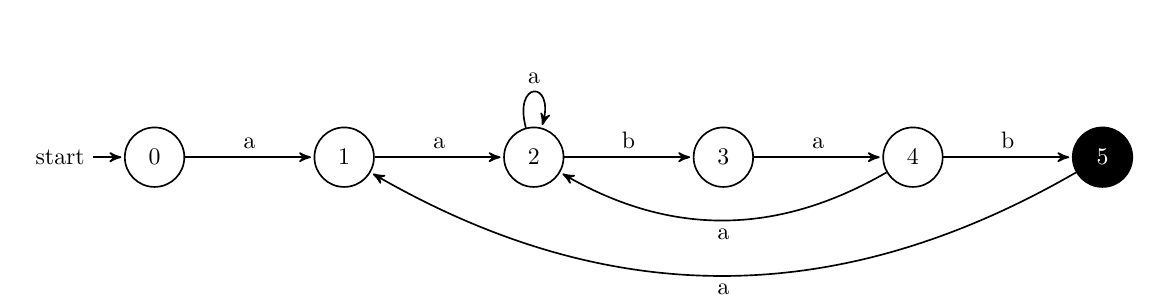
\begin{tikzpicture}[->,>=stealth',shorten >=1pt,auto,node distance=2.8cm,
                    semithick, scale=0.86, every node/.style={scale=0.86}]
  \tikzstyle{every state}=[fill=none,draw=black,text=black]

  \node[initial,state] (0)                    {$0$};
  \node[state]         (1) [right of=0] {$1$};
  \node[state]         (2) [right of=1] {$2$};
  \node[state]         (3) [right of=2] {$3$};
  \node[state]         (4) [right of=3]       {$4$};
  \node[state, fill=black, text=white]         (5) [right of=4]       {$5$};

  \path (0) edge node {a} (1)
        (1) edge node {a} (2)
        (2) edge [loop above] node {a} (2)
            edge node {b} (3)
        (3) edge node {a} (4)
        (4) edge node {b} (5)
              edge [bend left] node {a} (2) (5) edge [bend left] node {a} (1);
\end{tikzpicture}

Next, we illustrate its operation on the text string $T$.

\begin{center}
\begin{tabular} {| c | c |}
\hline
\textbf{Chars. consumed} & \textbf{State (current state in red)} \\
\hline
$a$ & {
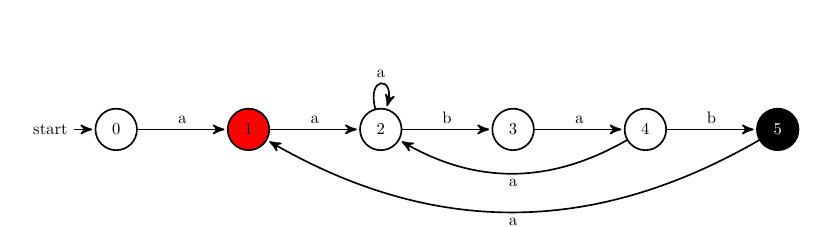
\begin{tikzpicture}[->,>=stealth',shorten >=1pt,auto,node distance=2.8cm,
                    semithick, scale=0.6, every node/.style={scale=0.6}]
  \tikzstyle{every state}=[fill=none,draw=black,text=black]

  \node[initial,state] (0)                    {$0$};
  \node[state, fill = red]         (1) [right of=0] {$1$};
  \node[state]         (2) [right of=1] {$2$};
  \node[state]         (3) [right of=2] {$3$};
  \node[state]         (4) [right of=3]       {$4$};
  \node[state, fill=black, text=white]         (5) [right of=4]       {$5$};

  \path (0) edge node {a} (1)
        (1) edge node {a} (2)
        (2) edge [loop above] node {a} (2)
            edge node {b} (3)
        (3) edge node {a} (4)
        (4) edge node {b} (5)
              edge [bend left] node {a} (2) (5) edge [bend left] node {a} (1);
\end{tikzpicture}
} \\
\hline

$aa$ & {
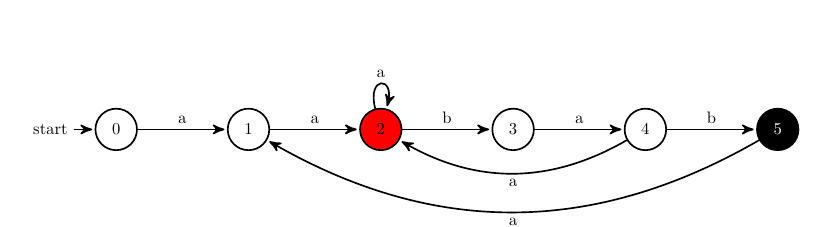
\begin{tikzpicture}[->,>=stealth',shorten >=1pt,auto,node distance=2.8cm,
                    semithick, scale=0.6, every node/.style={scale=0.6}]
  \tikzstyle{every state}=[fill=none,draw=black,text=black]

  \node[initial,state] (0)                    {$0$};
  \node[state]         (1) [right of=0] {$1$};
  \node[state, fill = red]         (2) [right of=1] {$2$};
  \node[state]         (3) [right of=2] {$3$};
  \node[state]         (4) [right of=3]       {$4$};
  \node[state, fill=black, text=white]         (5) [right of=4]       {$5$};

  \path (0) edge node {a} (1)
        (1) edge node {a} (2)
        (2) edge [loop above] node {a} (2)
            edge node {b} (3)
        (3) edge node {a} (4)
        (4) edge node {b} (5)
              edge [bend left] node {a} (2) (5) edge [bend left] node {a} (1);
\end{tikzpicture}
} \\
\hline

$aaa$ & {
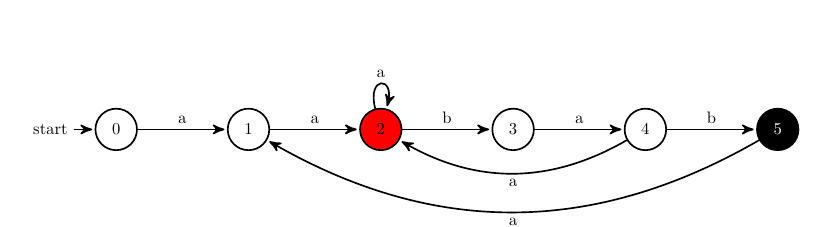
\begin{tikzpicture}[->,>=stealth',shorten >=1pt,auto,node distance=2.8cm,
                    semithick, scale=0.6, every node/.style={scale=0.6}]
  \tikzstyle{every state}=[fill=none,draw=black,text=black]

  \node[initial,state] (0)                    {$0$};
  \node[state]         (1) [right of=0] {$1$};
  \node[state, fill = red]         (2) [right of=1] {$2$};
  \node[state]         (3) [right of=2] {$3$};
  \node[state]         (4) [right of=3]       {$4$};
  \node[state, fill=black, text=white]         (5) [right of=4]       {$5$};

  \path (0) edge node {a} (1)
        (1) edge node {a} (2)
        (2) edge [loop above] node {a} (2)
            edge node {b} (3)
        (3) edge node {a} (4)
        (4) edge node {b} (5)
              edge [bend left] node {a} (2) (5) edge [bend left] node {a} (1);
\end{tikzpicture}
} \\
\hline

$aaab$ & {
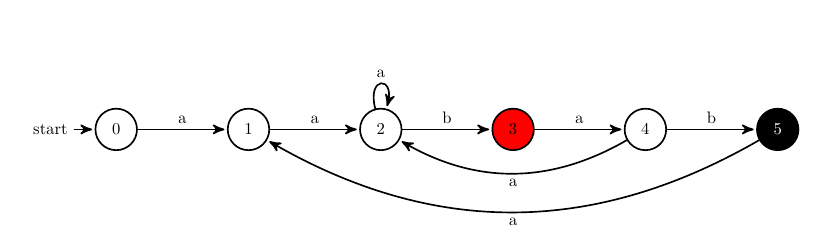
\begin{tikzpicture}[->,>=stealth',shorten >=1pt,auto,node distance=2.8cm,
                    semithick, scale=0.6, every node/.style={scale=0.6}]
  \tikzstyle{every state}=[fill=none,draw=black,text=black]

  \node[initial,state] (0)                    {$0$};
  \node[state]         (1) [right of=0] {$1$};
  \node[state]         (2) [right of=1] {$2$};
  \node[state, fill = red]         (3) [right of=2] {$3$};
  \node[state]         (4) [right of=3]       {$4$};
  \node[state, fill=black, text=white]         (5) [right of=4]       {$5$};

  \path (0) edge node {a} (1)
        (1) edge node {a} (2)
        (2) edge [loop above] node {a} (2)
            edge node {b} (3)
        (3) edge node {a} (4)
        (4) edge node {b} (5)
              edge [bend left] node {a} (2) (5) edge [bend left] node {a} (1);
\end{tikzpicture}
} \\
\hline

$aaaba$ & {
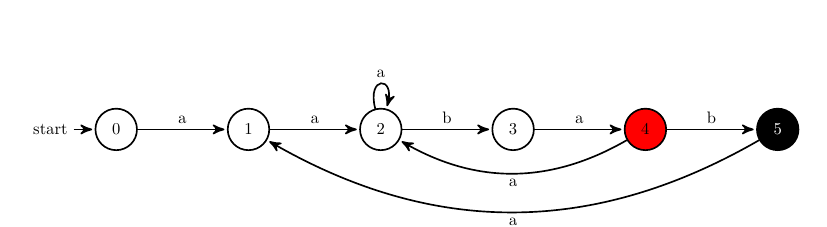
\begin{tikzpicture}[->,>=stealth',shorten >=1pt,auto,node distance=2.8cm,
                    semithick, scale=0.6, every node/.style={scale=0.6}]
  \tikzstyle{every state}=[fill=none,draw=black,text=black]

  \node[initial,state] (0)                    {$0$};
  \node[state]         (1) [right of=0] {$1$};
  \node[state]         (2) [right of=1] {$2$};
  \node[state]         (3) [right of=2] {$3$};
  \node[state, fill = red]         (4) [right of=3]       {$4$};
  \node[state, fill=black, text=white]         (5) [right of=4]       {$5$};

  \path (0) edge node {a} (1)
        (1) edge node {a} (2)
        (2) edge [loop above] node {a} (2)
            edge node {b} (3)
        (3) edge node {a} (4)
        (4) edge node {b} (5)
              edge [bend left] node {a} (2) (5) edge [bend left] node {a} (1);
\end{tikzpicture}
} \\
\hline

$aaabab$ & {
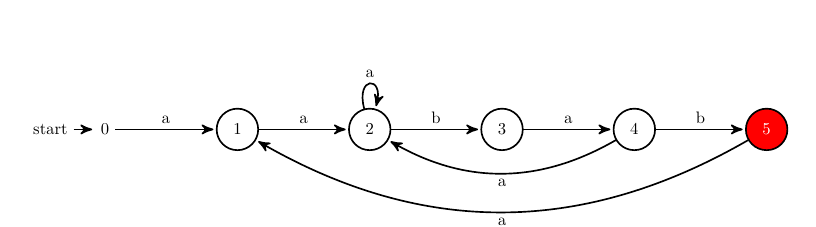
\begin{tikzpicture}[->,>=stealth',shorten >=1pt,auto,node distance=2.8cm,
                    semithick, scale=0.6, every node/.style={scale=0.6}]
  \tikzstyle{every state}=[fill=none,draw=black,text=black]

  \node[initial] (0)                    {$0$};
  \node[state]         (1) [right of=0] {$1$};
  \node[state]         (2) [right of=1] {$2$};
  \node[state]         (3) [right of=2] {$3$};
  \node[state]         (4) [right of=3]       {$4$};
  \node[state, fill=red, text=white]         (5) [right of=4]       {$5$};

  \path (0) edge node {a} (1)
        (1) edge node {a} (2)
        (2) edge [loop above] node {a} (2)
            edge node {b} (3)
        (3) edge node {a} (4)
        (4) edge node {b} (5)
              edge [bend left] node {a} (2) (5) edge [bend left] node {a} (1);
\end{tikzpicture}
} \\
\hline

$aaababa$ & {
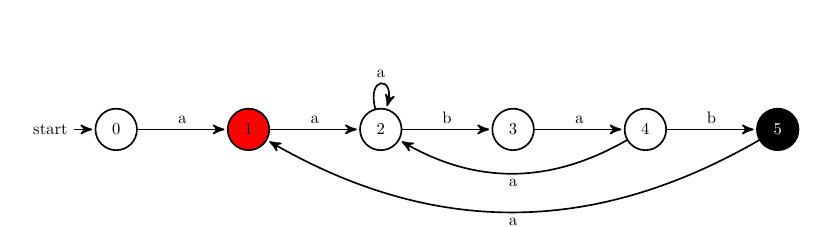
\begin{tikzpicture}[->,>=stealth',shorten >=1pt,auto,node distance=2.8cm,
                    semithick, scale=0.6, every node/.style={scale=0.6}]
  \tikzstyle{every state}=[fill=none,draw=black,text=black]

  \node[initial,state] (0)                    {$0$};
  \node[state,fill = red]         (1) [right of=0] {$1$};
  \node[state]         (2) [right of=1] {$2$};
  \node[state]         (3) [right of=2] {$3$};
  \node[state]         (4) [right of=3]       {$4$};
  \node[state, fill=black, text=white]         (5) [right of=4]       {$5$};

  \path (0) edge node {a} (1)
        (1) edge node {a} (2)
        (2) edge [loop above] node {a} (2)
            edge node {b} (3)
        (3) edge node {a} (4)
        (4) edge node {b} (5)
              edge [bend left] node {a} (2) (5) edge [bend left] node {a} (1);
\end{tikzpicture}
} \\
\hline

$aaababaa$ & {
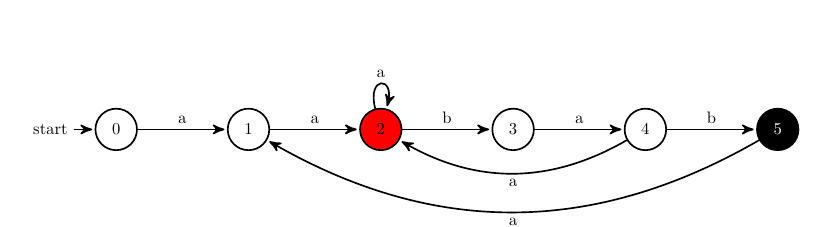
\begin{tikzpicture}[->,>=stealth',shorten >=1pt,auto,node distance=2.8cm,
                    semithick, scale=0.6, every node/.style={scale=0.6}]
  \tikzstyle{every state}=[fill=none,draw=black,text=black]

  \node[initial,state] (0)                    {$0$};
  \node[state]         (1) [right of=0] {$1$};
  \node[state,fill = red]         (2) [right of=1] {$2$};
  \node[state]         (3) [right of=2] {$3$};
  \node[state]         (4) [right of=3]       {$4$};
  \node[state, fill=black, text=white]         (5) [right of=4]       {$5$};

  \path (0) edge node {a} (1)
        (1) edge node {a} (2)
        (2) edge [loop above] node {a} (2)
            edge node {b} (3)
        (3) edge node {a} (4)
        (4) edge node {b} (5)
              edge [bend left] node {a} (2) (5) edge [bend left] node {a} (1);
\end{tikzpicture}
} \\
\hline

$aaababaab$ & {
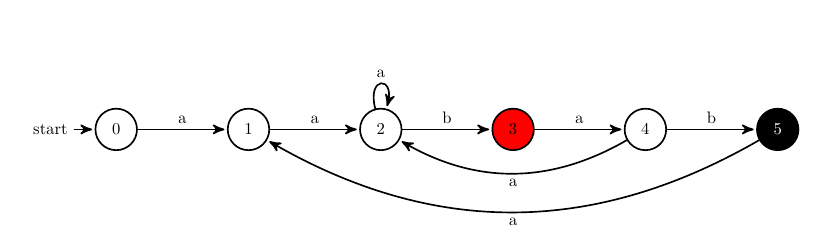
\begin{tikzpicture}[->,>=stealth',shorten >=1pt,auto,node distance=2.8cm,
                    semithick, scale=0.6, every node/.style={scale=0.6}]
  \tikzstyle{every state}=[fill=none,draw=black,text=black]

  \node[initial,state] (0)                    {$0$};
  \node[state]         (1) [right of=0] {$1$};
  \node[state]         (2) [right of=1] {$2$};
  \node[state,fill = red]         (3) [right of=2] {$3$};
  \node[state]         (4) [right of=3]       {$4$};
  \node[state, fill=black, text=white]         (5) [right of=4]       {$5$};

  \path (0) edge node {a} (1)
        (1) edge node {a} (2)
        (2) edge [loop above] node {a} (2)
            edge node {b} (3)
        (3) edge node {a} (4)
        (4) edge node {b} (5)
              edge [bend left] node {a} (2) (5) edge [bend left] node {a} (1);
\end{tikzpicture}
} \\
\hline

\end{tabular}

\begin{tabular} {| c | c |}

\hline
$aaababaaba$ & {
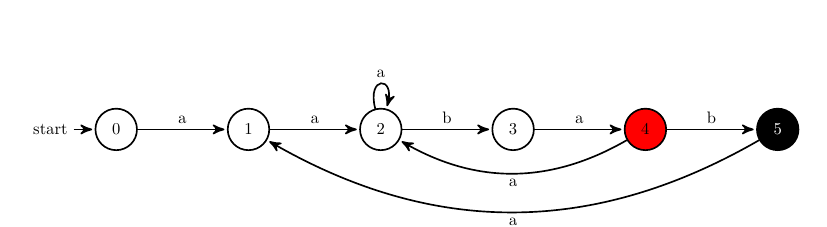
\begin{tikzpicture}[->,>=stealth',shorten >=1pt,auto,node distance=2.8cm,
                    semithick, scale=0.6, every node/.style={scale=0.6}]
  \tikzstyle{every state}=[fill=none,draw=black,text=black]

  \node[initial,state] (0)                    {$0$};
  \node[state]         (1) [right of=0] {$1$};
  \node[state]         (2) [right of=1] {$2$};
  \node[state]         (3) [right of=2] {$3$};
  \node[state,fill = red]         (4) [right of=3]       {$4$};
  \node[state, fill=black, text=white]         (5) [right of=4]       {$5$};

  \path (0) edge node {a} (1)
        (1) edge node {a} (2)
        (2) edge [loop above] node {a} (2)
            edge node {b} (3)
        (3) edge node {a} (4)
        (4) edge node {b} (5)
              edge [bend left] node {a} (2) (5) edge [bend left] node {a} (1);
\end{tikzpicture}
} \\
\hline
$aaababaabaa$ & {
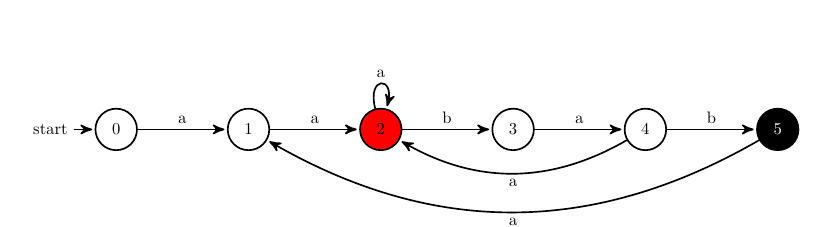
\begin{tikzpicture}[->,>=stealth',shorten >=1pt,auto,node distance=2.8cm,
                    semithick, scale=0.6, every node/.style={scale=0.6}]
  \tikzstyle{every state}=[fill=none,draw=black,text=black]

  \node[initial,state] (0)                    {$0$};
  \node[state]         (1) [right of=0] {$1$};
  \node[state,fill = red]         (2) [right of=1] {$2$};
  \node[state]         (3) [right of=2] {$3$};
  \node[state]         (4) [right of=3]       {$4$};
  \node[state, fill=black, text=white]         (5) [right of=4]       {$5$};

  \path (0) edge node {a} (1)
        (1) edge node {a} (2)
        (2) edge [loop above] node {a} (2)
            edge node {b} (3)
        (3) edge node {a} (4)
        (4) edge node {b} (5)
              edge [bend left] node {a} (2) (5) edge [bend left] node {a} (1);
\end{tikzpicture}
} \\

\hline
$aaababaabaab$ & {
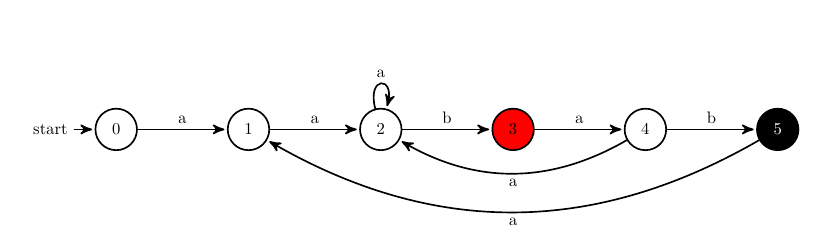
\begin{tikzpicture}[->,>=stealth',shorten >=1pt,auto,node distance=2.8cm,
                    semithick, scale=0.6, every node/.style={scale=0.6}]
  \tikzstyle{every state}=[fill=none,draw=black,text=black]

  \node[initial,state] (0)                    {$0$};
  \node[state]         (1) [right of=0] {$1$};
  \node[state]         (2) [right of=1] {$2$};
  \node[state,fill = red]         (3) [right of=2] {$3$};
  \node[state]         (4) [right of=3]       {$4$};
  \node[state, fill=black, text=white]         (5) [right of=4]       {$5$};

  \path (0) edge node {a} (1)
        (1) edge node {a} (2)
        (2) edge [loop above] node {a} (2)
            edge node {b} (3)
        (3) edge node {a} (4)
        (4) edge node {b} (5)
              edge [bend left] node {a} (2) (5) edge [bend left] node {a} (1);
\end{tikzpicture}
} \\
\hline

$aaababaabaaba$ & {
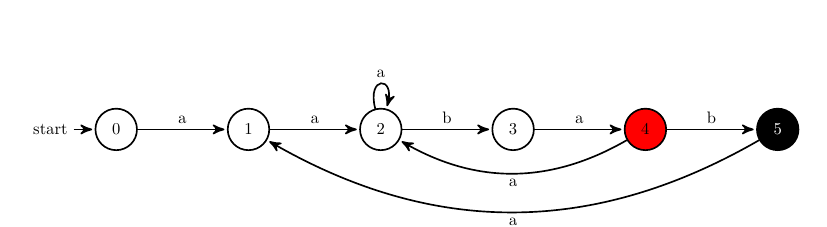
\begin{tikzpicture}[->,>=stealth',shorten >=1pt,auto,node distance=2.8cm,
                    semithick, scale=0.6, every node/.style={scale=0.6}]
  \tikzstyle{every state}=[fill=none,draw=black,text=black]

  \node[initial,state] (0)                    {$0$};
  \node[state]         (1) [right of=0] {$1$};
  \node[state]         (2) [right of=1] {$2$};
  \node[state]         (3) [right of=2] {$3$};
  \node[state,fill = red]         (4) [right of=3]       {$4$};
  \node[state, fill=black, text=white]         (5) [right of=4]       {$5$};

  \path (0) edge node {a} (1)
        (1) edge node {a} (2)
        (2) edge [loop above] node {a} (2)
            edge node {b} (3)
        (3) edge node {a} (4)
        (4) edge node {b} (5)
              edge [bend left] node {a} (2) (5) edge [bend left] node {a} (1);
\end{tikzpicture}
} \\
\hline

$aaababaabaabab$ & {
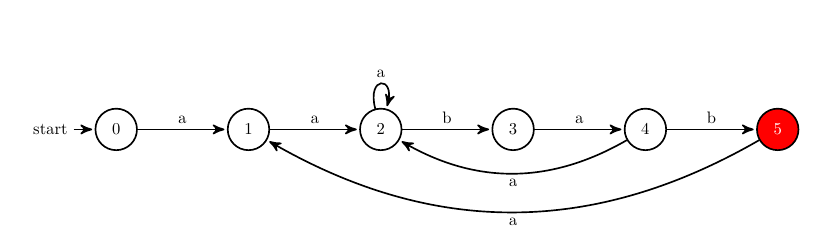
\begin{tikzpicture}[->,>=stealth',shorten >=1pt,auto,node distance=2.8cm,
                    semithick, scale=0.6, every node/.style={scale=0.6}]
  \tikzstyle{every state}=[fill=none,draw=black,text=black]

  \node[initial,state] (0)                    {$0$};
  \node[state]         (1) [right of=0] {$1$};
  \node[state]         (2) [right of=1] {$2$};
  \node[state]         (3) [right of=2] {$3$};
  \node[state]         (4) [right of=3]       {$4$};
  \node[state,fill = red, text=white]         (5) [right of=4]       {$5$};

  \path (0) edge node {a} (1)
        (1) edge node {a} (2)
        (2) edge [loop above] node {a} (2)
            edge node {b} (3)
        (3) edge node {a} (4)
        (4) edge node {b} (5)
              edge [bend left] node {a} (2) (5) edge [bend left] node {a} (1);
\end{tikzpicture}
} \\
\hline

$aaababaabaababa$ & {
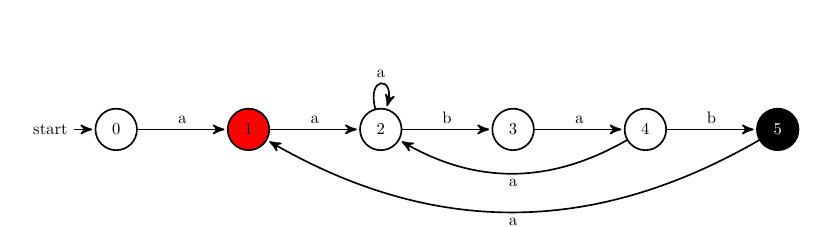
\begin{tikzpicture}[->,>=stealth',shorten >=1pt,auto,node distance=2.8cm,
                    semithick, scale=0.6, every node/.style={scale=0.6}]
  \tikzstyle{every state}=[fill=none,draw=black,text=black]

  \node[initial,state] (0)                    {$0$};
  \node[state, fill = red]         (1) [right of=0] {$1$};
  \node[state]         (2) [right of=1] {$2$};
  \node[state]         (3) [right of=2] {$3$};
  \node[state]         (4) [right of=3]       {$4$};
  \node[state,fill = black, text=white]         (5) [right of=4]       {$5$};

  \path (0) edge node {a} (1)
        (1) edge node {a} (2)
        (2) edge [loop above] node {a} (2)
            edge node {b} (3)
        (3) edge node {a} (4)
        (4) edge node {b} (5)
              edge [bend left] node {a} (2) (5) edge [bend left] node {a} (1);
\end{tikzpicture}
} \\
\hline

$aaababaabaababaa$ & {
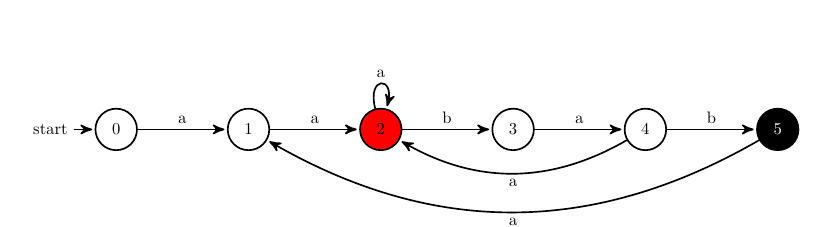
\begin{tikzpicture}[->,>=stealth',shorten >=1pt,auto,node distance=2.8cm,
                    semithick, scale=0.6, every node/.style={scale=0.6}]
  \tikzstyle{every state}=[fill=none,draw=black,text=black]

  \node[initial,state] (0)                    {$0$};
  \node[state]         (1) [right of=0] {$1$};
  \node[state, fill = red]         (2) [right of=1] {$2$};
  \node[state]         (3) [right of=2] {$3$};
  \node[state]         (4) [right of=3]       {$4$};
  \node[state,fill = black, text=white]         (5) [right of=4]       {$5$};

  \path (0) edge node {a} (1)
        (1) edge node {a} (2)
        (2) edge [loop above] node {a} (2)
            edge node {b} (3)
        (3) edge node {a} (4)
        (4) edge node {b} (5)
              edge [bend left] node {a} (2) (5) edge [bend left] node {a} (1);
\end{tikzpicture}
} \\
\hline

$aaababaabaababaab$ & {
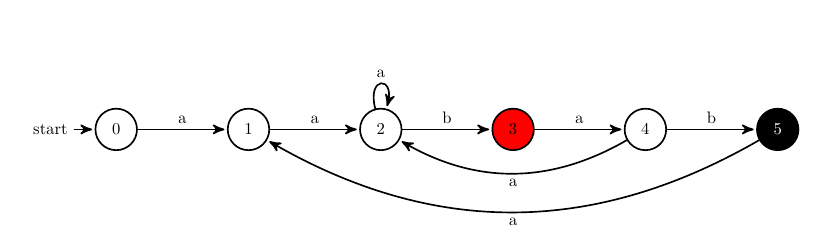
\begin{tikzpicture}[->,>=stealth',shorten >=1pt,auto,node distance=2.8cm,
                    semithick, scale=0.6, every node/.style={scale=0.6}]
  \tikzstyle{every state}=[fill=none,draw=black,text=black]

  \node[initial,state] (0)                    {$0$};
  \node[state]         (1) [right of=0] {$1$};
  \node[state]         (2) [right of=1] {$2$};
  \node[state, fill = red]         (3) [right of=2] {$3$};
  \node[state]         (4) [right of=3]       {$4$};
  \node[state,fill = black, text=white]         (5) [right of=4]       {$5$};

  \path (0) edge node {a} (1)
        (1) edge node {a} (2)
        (2) edge [loop above] node {a} (2)
            edge node {b} (3)
        (3) edge node {a} (4)
        (4) edge node {b} (5)
              edge [bend left] node {a} (2) (5) edge [bend left] node {a} (1);
\end{tikzpicture}
} \\
\hline

\end{tabular}
\end{center}

%----------------------------------------------------------------------------------------
%	PROBLEM 5
%----------------------------------------------------------------------------------------

\section{Automaton structure for non-overlappable patterns}

We call a pattern $P$ \emph{nonoverlappable} if $P_k \sqsupset P_q$ implies $k = 0$ or $k = q$. We describe the state-transition diagram of the string-matching automaton for a nonoverlappable pattern.\\

First, here's a graph (partially) showing the state-transition diagram of the string-matching automaton for a nonoverlappable. A full justification of this diagram is given below:

\begin{center}
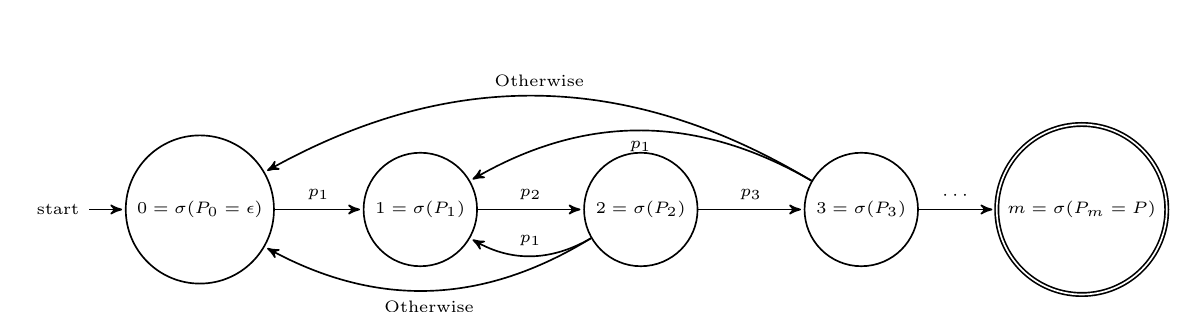
\begin{tikzpicture}[->,>=stealth',shorten >=1pt,auto,node distance=2.8cm,
                    semithick]
\tikzstyle{every state}=[fill=none,draw=black,text=black]
\tikzset{font=\fontsize{6pt}{12}\selectfont}
  
        \node[state,initial]                (0)                           {$0 = \sigma(P_0 = \epsilon)$};
        \node[state]                        (1)   [right of=0]          {$1 = \sigma(P_1)$};
        \node[state]                        (2)   [right of=1]          {$2 = \sigma(P_2)$};
        \node[state]                        (3)   [right of=2]          {$3 = \sigma(P_3)$};
        \node[state,accepting]              (4)   [right of =3]          {$m= \sigma(P_m = P)$};    

        \path[->]
        (0)   edge                        node {$p_1$}            (1)  
        (1)   edge                        node {$p_2$}            (2) 
        (2)   edge                        node {$p_3$}          (3) 
        (2)   edge [bend left, above] 	     node {$p_1$}          (1) 
        (2)   edge [bend left] 	     node {Otherwise}          (0) 
        (3)   edge [bend right, below] 	     node {$p_1$}          (1) 
        (3)   edge [bend right, above] 	     node {Otherwise}          (0) 
        (3)   edge                        node {$\cdots$}          (4) 
        ; %end path 
\end{tikzpicture}  
\end{center}

To see this diagram is in fact correct, first note if $P_k \sqsupset P_q$ implies $k = 0$ or $k = q$, then the first character in the pattern must be unique (i.e. $p_1 \ne p_j$ for $j = 2, \cdots, m$, where $m = |P|$). If not, then there is some $P_q, q \ne 1$, such that $P_1 \sqsupset P_q$, which is a contradiction.\\

But then, given a state $P_k$ (with $\sigma(P_k) = k$),

\[
\delta(P_k, a) =
\begin{cases}
\sigma(P_{k + 1}) & \textrm{ if } a = p_{k + 1} \\
\sigma(P_{1}) & \textrm{ if } a = p_{1} \\
\sigma(P_{0}) & \textrm{ otherwise } \\
\end{cases}
\]

We justify each of these cases in turn:
\begin{itemize}
\item $\delta(P_k, a) = \sigma(P_{k + 1}) \textrm{ if } a = p_{k + 1}$: Note by CLRS definition 32.4, $delta(P_k, p_{k+1}) = \sigma(P_{k}p_{k+1}) = \sigma(P_{k + 1})$.
\item $\delta(P_k, a) = \sigma(P_{1}) \textrm{ if } a = p_{1}$: We show this by contradiction. If, for some $k > 1$, $\delta(P_k, p_{1}) \ne \sigma(P_{1})$, then $\delta(P_k, p_{1}) = P_j = p_1 \cdots p_{j-1} p_1$ (noting that obviously $j \geq 1$, and by assumption $j \ne 1$). But then $p_1$ is not unique in $P$, yielding a contradiction. Hence $\delta(P_k, p_{1}) = \sigma(P_{1})$.
\item $\delta(P_k, a) = \sigma(P_{0}) \textrm{ otherwise}$: Again we show this by contradiction. If, for some $k$ and some $a \ne p_1$ or $p_{k+1}$, $\delta(P_k, a) = \sigma(P_k a) = \sigma(P_j)$ for some $j > 1$, then we must have $P_{j-1} \sqsupset P_k$, yielding our contradition. Hence $\delta(P_k, a) = \sigma(P_{0})$ for all $a \ne p_{k+1}, p_{1}$.
\end{itemize}

%----------------------------------------------------------------------------------------
%	PROBLEM 6
%----------------------------------------------------------------------------------------

\section{Prefix function}

Below is the prefix function $\pi$ for the pattern $ababbabbabbababbabb$.

\begin{center}
\begin{tabular}{| l | c | c |}
\hline
\textbf{Prefix} &\textbf{$q$ (i.e. input to prefix function $\pi$)} & $\pi[q]$ \\
\hline
$a$ & 1 & 0 \\
\hline
$ab$ & 2 & 0 \\
\hline
$aba$ & 3 & 1 \\
\hline
$abab$ & 4 & 2 \\
\hline
$ababb$ & 5 & 0 \\
\hline
$ababba$ & 6 & 1 \\
\hline
$ababbab$ & 7 & 2 \\
\hline
$ababbabb$ & 8 & 0 \\
\hline
$ababbabba$ & 9 & 1 \\
\hline
$ababbabbab$ & 10 & 2 \\
\hline
$ababbabbabb$ & 11 & 0 \\
\hline
$ababbabbabba$ & 12 & 1 \\
\hline
$ababbabbabbab$ & 13 & 2 \\
\hline
$ababbabbabbaba$ & 14 & 3 \\
\hline
$ababbabbabbabab$ & 15 & 4 \\
\hline
$ababbabbabbababb$ & 16 & 5 \\
\hline
$ababbabbabbababba$ & 17 & 6 \\
\hline
$ababbabbabbababbab$ & 18 & 7 \\
\hline
$ababbabbabbababbabb$ & 19 & 8 \\
\hline
\end{tabular}
\end{center}

%----------------------------------------------------------------------------------------
%	PROBLEM 7
%----------------------------------------------------------------------------------------

\section{Linear-time algorithm to determine if $T$ is a cyclic rotation of $T'$}

We give a linear-time algorithm to determine whether a text $T$ is a cyclic rotation of another string $T'$. For example, arc and car are cyclic rotations of each other.

\begin{algorithmic}
\Function{cyclic\_rotation}{$T, T'$}
	\State $T'' = T + T$ \Comment{+ is the string concatenation operator}
	\State \texttt{KMP-Matcher}($T'', T'$)
\EndFunction
\end{algorithmic}

Note this is a linear-time algorithm, since
\begin{itemize}
\item String concatenation is assumed to be a linear time operation $O(n)$
\item Inside \texttt{KMP-Matcher}, \texttt{compute-prefix-function}($T$) runs in $O(n)$ time
\item The rest of \texttt{KMP-Matcher} runs in $O(2n) = O(n)$ time
\end{itemize}

Moreover, this is algorithm is clearly correct, since if $T$ and $T'$ are cyclic rotations of each other, then $T'$ is a substring of $T" = T + T$, so the algorithm finds the cyclic rotation required to match the strings.

%----------------------------------------------------------------------------------------
%	PROBLEM 8
%----------------------------------------------------------------------------------------

\section{Longest palindromic substring}

The longest palindromic substring is a maximum-length contiguous substring of a given string that is a palindrome. For example, the longest palindromic substring of $ultramarine$ is $ramar$. \\

We give an efficient algorithm to determine the longest palindromic substring of a given string, then we explain the algorithm and illustrate its operation on the string $evenness$. First, we present the algorithm (Manacher's Algorithm). The basic idea of this algorithm is to iterate from left to right in (a preprocessed version) of the input string. As we iterate, we  store information about previously seen palindromes. In particular, we keep track of the known palindrome that extends furthest to the right. By storing this information, we can exploit the inherent symmetry of palindromes to reduce the total number of comparisons necessary to identify the longest palindromic substring, and achieve a runtime of $O(n)$. The algorithm is: \\

\begin{algorithmic}
\Function{longest\_palindrome}{S}
	\State S2 = \texttt{preprocess}(S)
	\State P = array of zeros with length(S2)
	\State C = 1 \Comment{Position of current palindrome center}
	\State R = 1 \Comment{Position of right boundary of current palindrome}
	\For {i = 2 to length(S2) - 1}
		\State m = 2C - 1 \Comment{Position of mirror element across current palindrome center}
		\If {i < R} \Comment{Case 1- see explanation}
			\If {R - i > P[m]} \Comment{Case 1a - see explanation}
				\State P[i] = P[m]
			\Else \Comment{Case 1b- see explanation}
				\State P[i] = R - i
				\While {S2[i - (1 + P[i])] == S2[i + (1 + P[i])]}
					\State P[i] ++
				\EndWhile
				\If {i + P[i] > R}
					\State C = i
					\State R = i + P[i]
				\EndIf
			\EndIf
		\Else \Comment{Case 2- see explanation}
			\While {S2[i - (1 + P[i])] == S2[i + (1 + P[i])]}
					\State P[i] ++
			\EndWhile
			\If {i + P[i] > R}
				\State C = i
				\State R = i + P[i]
			\EndIf
		\EndIf
	\EndFor
	\State \Return \texttt{palindrome\_from\_span}(S2, P)
\EndFunction
\end{algorithmic}

Before giving pseudocode for the helper functions \texttt{palindrome\_from\_span} and \texttt{preprocess}, we explain the logic behind this algorithm:
\begin{itemize}
\item \textbf{Case 1a}: In this case, by symmetry, P[i] = P[m]. This is because the palindromes centered on \texttt{m} (and by symmetry on \texttt{i}) are both fully contained within the palindrome centered on \texttt{c}, and thus are identical.
\item \textbf{Case 1b}: In this case, the palindrome centered on \texttt{m} goes at least to the left edge of the current palindrome (centered on \texttt{c}). Hence, by symmetry, the palindrome centered on \texttt{i} extends as least as far as \texttt{R}, but it may extend further. Thus, we need to make additional comparisons (past \texttt{R}), and potentially update \texttt{C} and \texttt{R} (if we find a palindrome that extends past \texttt{R}).   
\item \textbf{Case 2}: In this case, \texttt{i} is outside the current palindrome (past \texttt{R}) and thus we don't know anything about \texttt{P[i]}. Thus we immediately begin making comparisons and potentially update \texttt{C} and \texttt{R}.
\end{itemize}

Now that we've presented and explained the main algorithm, we present psuedocode for the two helper functions, then illustrate the operation of the algorithm on the string $evenness$. \\

\begin{algorithmic}
\Function{preprocess}{S}
	\State S = insert '\#' between every character in S
	\State S2 = '\$\#' + S + '@'
	\State \Return S2
\EndFunction
\end{algorithmic}

\begin{algorithmic}
\Function{palindrome\_from\_span}{S2, P}
	\State max\_span = max(P)
	\State max\_center = index of max\_span in P
	\State start = max\_center - max\_span + 1 \Comment{+1 since palindrome starts with '\#'}
	\State stop = max\_center + max\_span
	\State result = new String
	\State next\_char = start
	\While {next\_char < stop}
		\State result = result + S2[next\_char] \Comment{Add next\_char to result}
		\State next\_char = next\_char + 2
	\EndWhile
	\State \Return result
\EndFunction
\end{algorithmic}

\begin{center}
\begin{tabular}{| c | p {14 cm} |}
\hline
\texttt{i}  & 
Diagram showing algorithm operation.
\begin{itemize}
\item The pointers for \texttt{C,R, m}, and the current position \texttt{i} shown in blue indicate the state when the \texttt{for} loop is entered. 
\item The \texttt{while} loop comparisons that match are shown in orange, and those that don't match are shown in green.
\item The final incremented palindrome length \texttt{P[i]} (i.e. the state when control leaves the \texttt{while} loop) is drawn above.
\end{itemize}
\\
\hline

%---------------------------------------------------------------------------------------------------------------------------------------%
2 &

~

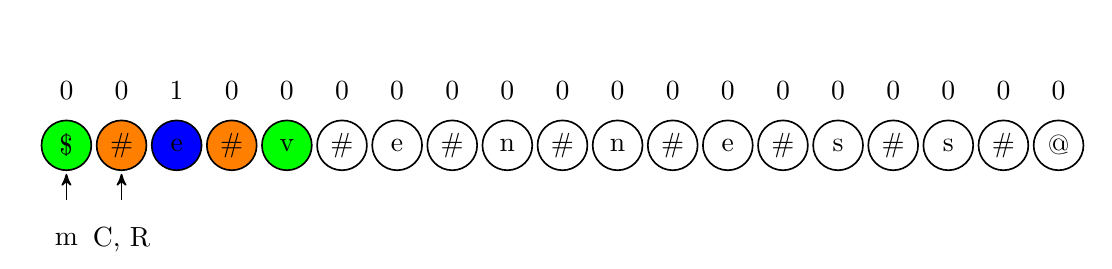
\begin{tikzpicture}[->,>=stealth',shorten >=1pt,auto,node distance=0.7cm,
                    semithick]
\tikzstyle{every state}=[fill=none,draw=black,text=black]
\tikzset{font=\fontsize{10pt}{12}\selectfont}

  
        \node[state,inner sep=2pt,minimum size=18pt, fill=green]                (0)                           {\$};
        \node[state,inner sep=2pt,minimum size=18pt, draw=none]                (p0) [above of=0] {0};
        
        \node[state,inner sep=2pt,minimum size=18pt, fill=orange]                        (1)   [right of=0]          {\#};
        \node[state,inner sep=2pt,minimum size=18pt, draw=none]                (p1) [above of=1] {0};
        
        \node[state,inner sep=2pt,minimum size=18pt, fill=blue]                        (2)   [right of=1]          {e};
        \node[state,inner sep=2pt,minimum size=18pt, draw=none]                (p2) [above of=2] {1};
        
        \node[state,inner sep=2pt,minimum size=18pt, fill=orange]                        (3)   [right of=2]          {\#};
        \node[state,inner sep=2pt,minimum size=18pt, draw=none]                (p3) [above of=3] {0};
        
        \node[state,inner sep=2pt,minimum size=18pt, fill=green]              (4)   [right of=3]          {v}; 
        \node[state,inner sep=2pt,minimum size=18pt, draw=none]                (p4) [above of=4] {0};
           
        \node[state,inner sep=2pt,minimum size=18pt]                        (5)   [right of=4]          {\#};
        \node[state,inner sep=2pt,minimum size=18pt, draw=none]                (p5) [above of=5] {0};
        
        \node[state,inner sep=2pt,minimum size=18pt]                        (6)   [right of=5]          {e};
        \node[state,inner sep=2pt,minimum size=18pt, draw=none]                (p6) [above of=6] {0};
        
        \node[state,inner sep=2pt,minimum size=18pt]                        (7)   [right of=6]          {\#};
        \node[state,inner sep=2pt,minimum size=18pt, draw=none]                (p7) [above of=7] {0};
        
        \node[state,inner sep=2pt,minimum size=18pt]              (8)   [right of=7]          {n};
        \node[state,inner sep=2pt,minimum size=18pt, draw=none]                (p8) [above of=8] {0};
            
        \node[state,inner sep=2pt,minimum size=18pt]                        (9)   [right of=8]          {\#};
        \node[state,inner sep=2pt,minimum size=18pt, draw=none]                (p9) [above of=9] {0};
        
        \node[state,inner sep=2pt,minimum size=18pt]                        (10)   [right of=9]          {n};
        \node[state,inner sep=2pt,minimum size=18pt, draw=none]                (p10) [above of=10] {0};
        
        \node[state,inner sep=2pt,minimum size=18pt]                        (11)   [right of=10]          {\#};
        \node[state,inner sep=2pt,minimum size=18pt, draw=none]                (p11) [above of=11] {0};
        
        \node[state,inner sep=2pt,minimum size=18pt]                        (12)   [right of=11]          {e};
        \node[state,inner sep=2pt,minimum size=18pt, draw=none]                (p12) [above of=12] {0};
        
        \node[state,inner sep=2pt,minimum size=18pt]                        (13)   [right of=12]          {\#};
        \node[state,inner sep=2pt,minimum size=18pt, draw=none]                (p13) [above of=13] {0};
        
        \node[state,inner sep=2pt,minimum size=18pt]              (14)   [right of=13]          {s};
        \node[state,inner sep=2pt,minimum size=18pt, draw=none]                (p14) [above of=14] {0};
            
        \node[state,inner sep=2pt,minimum size=18pt]                        (15)   [right of=14]          {\#};
        \node[state,inner sep=2pt,minimum size=18pt, draw=none]                (p15) [above of=15] {0};
        
        \node[state,inner sep=2pt,minimum size=18pt]                        (16)   [right of=15]          {s};
        \node[state,inner sep=2pt,minimum size=18pt, draw=none]                (p16) [above of=16] {0};
        
        \node[state,inner sep=2pt,minimum size=18pt]                        (17)   [right of=16]          {\#};
        \node[state,inner sep=2pt,minimum size=18pt, draw=none]                (p17) [above of=17] {0};
        
        \node[state,inner sep=2pt,minimum size=18pt]                        (18)   [right of=17]          {@};
        \node[state,inner sep=2pt,minimum size=18pt, draw=none]                (p18) [above of=18] {0};
        
        \node[state,inner sep=2pt,minimum size=28pt,draw=none, node distance = 1.2 cm]	     (C) [below of=1] {C, R};
        %\node[state,inner sep=2pt,minimum size=28pt,draw=none, node distance = 1.2 cm]	     (R) [below of=1] {R};
        \node[state,inner sep=2pt,minimum size=28pt,draw=none, node distance = 1.2 cm]	     (m) [below of=0] {m};        
 
        \path[->]
        (C)   edge node {}            (1)  
        %(R)   edge node {}            (1)
        (m)   edge node {}          (0) 
        ; %end path 
        
\end{tikzpicture} 

\\

\hline

%---------------------------------------------------------------------------------------------------------------------------------------%

3 &

~

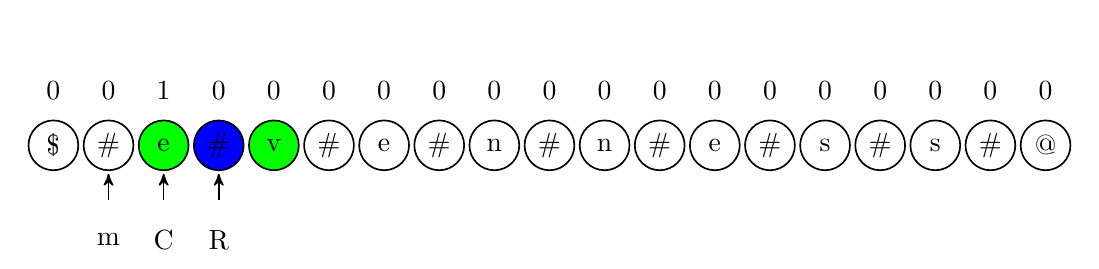
\begin{tikzpicture}[->,>=stealth',shorten >=1pt,auto,node distance=0.7cm,
                    semithick]
\tikzstyle{every state}=[fill=none,draw=black,text=black]
\tikzset{font=\fontsize{10pt}{12}\selectfont}

  
        \node[state,inner sep=2pt,minimum size=18pt]                (0)                           {\$};
        \node[state,inner sep=2pt,minimum size=18pt, draw=none]                (p0) [above of=0] {0};
        
        \node[state,inner sep=2pt,minimum size=18pt]                        (1)   [right of=0]          {\#};
        \node[state,inner sep=2pt,minimum size=18pt, draw=none]                (p1) [above of=1] {0};
        
        \node[state,inner sep=2pt,minimum size=18pt, fill=green]                        (2)   [right of=1]          {e};
        \node[state,inner sep=2pt,minimum size=18pt, draw=none]                (p2) [above of=2] {1};
        
        \node[state,inner sep=2pt,minimum size=18pt, fill=blue]                        (3)   [right of=2]          {\#};
        \node[state,inner sep=2pt,minimum size=18pt, draw=none]                (p3) [above of=3] {0};
        
        \node[state,inner sep=2pt,minimum size=18pt, fill=green]              (4)   [right of=3]          {v}; 
        \node[state,inner sep=2pt,minimum size=18pt, draw=none]                (p4) [above of=4] {0};
           
        \node[state,inner sep=2pt,minimum size=18pt]                        (5)   [right of=4]          {\#};
        \node[state,inner sep=2pt,minimum size=18pt, draw=none]                (p5) [above of=5] {0};
        
        \node[state,inner sep=2pt,minimum size=18pt]                        (6)   [right of=5]          {e};
        \node[state,inner sep=2pt,minimum size=18pt, draw=none]                (p6) [above of=6] {0};
        
        \node[state,inner sep=2pt,minimum size=18pt]                        (7)   [right of=6]          {\#};
        \node[state,inner sep=2pt,minimum size=18pt, draw=none]                (p7) [above of=7] {0};
        
        \node[state,inner sep=2pt,minimum size=18pt]              (8)   [right of=7]          {n};
        \node[state,inner sep=2pt,minimum size=18pt, draw=none]                (p8) [above of=8] {0};
            
        \node[state,inner sep=2pt,minimum size=18pt]                        (9)   [right of=8]          {\#};
        \node[state,inner sep=2pt,minimum size=18pt, draw=none]                (p9) [above of=9] {0};
        
        \node[state,inner sep=2pt,minimum size=18pt]                        (10)   [right of=9]          {n};
        \node[state,inner sep=2pt,minimum size=18pt, draw=none]                (p10) [above of=10] {0};
        
        \node[state,inner sep=2pt,minimum size=18pt]                        (11)   [right of=10]          {\#};
        \node[state,inner sep=2pt,minimum size=18pt, draw=none]                (p11) [above of=11] {0};
        
        \node[state,inner sep=2pt,minimum size=18pt]                        (12)   [right of=11]          {e};
        \node[state,inner sep=2pt,minimum size=18pt, draw=none]                (p12) [above of=12] {0};
        
        \node[state,inner sep=2pt,minimum size=18pt]                        (13)   [right of=12]          {\#};
        \node[state,inner sep=2pt,minimum size=18pt, draw=none]                (p13) [above of=13] {0};
        
        \node[state,inner sep=2pt,minimum size=18pt]              (14)   [right of=13]          {s};
        \node[state,inner sep=2pt,minimum size=18pt, draw=none]                (p14) [above of=14] {0};
            
        \node[state,inner sep=2pt,minimum size=18pt]                        (15)   [right of=14]          {\#};
        \node[state,inner sep=2pt,minimum size=18pt, draw=none]                (p15) [above of=15] {0};
        
        \node[state,inner sep=2pt,minimum size=18pt]                        (16)   [right of=15]          {s};
        \node[state,inner sep=2pt,minimum size=18pt, draw=none]                (p16) [above of=16] {0};
        
        \node[state,inner sep=2pt,minimum size=18pt]                        (17)   [right of=16]          {\#};
        \node[state,inner sep=2pt,minimum size=18pt, draw=none]                (p17) [above of=17] {0};
        
        \node[state,inner sep=2pt,minimum size=18pt]                        (18)   [right of=17]          {@};
        \node[state,inner sep=2pt,minimum size=18pt, draw=none]                (p18) [above of=18] {0};
        
        \node[state,inner sep=2pt,minimum size=28pt,draw=none, node distance = 1.2 cm]	     (C) [below of=2] {C};
        \node[state,inner sep=2pt,minimum size=28pt,draw=none, node distance = 1.2 cm]	     (R) [below of=3] {R};
        \node[state,inner sep=2pt,minimum size=28pt,draw=none, node distance = 1.2 cm]	     (m) [below of=1] {m};        
 
        \path[->]
        (C)   edge node {}            (2)  
        (R)   edge node {}            (3)
        (m)   edge node {}          (1) 
        ; %end path 
        
\end{tikzpicture} 

\\

\hline

%---------------------------------------------------------------------------------------------------------------------------------------%

4 &

~

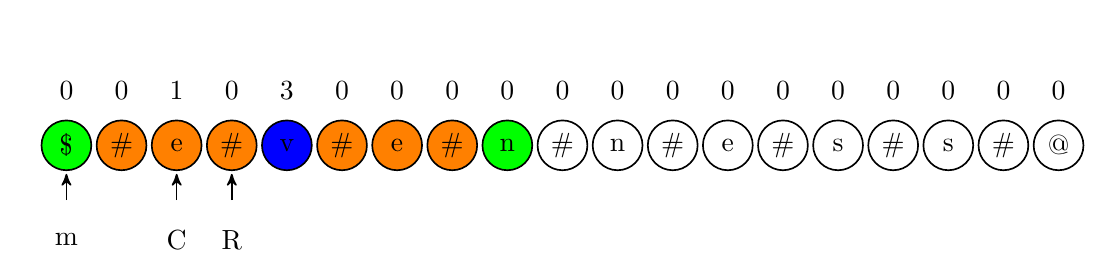
\begin{tikzpicture}[->,>=stealth',shorten >=1pt,auto,node distance=0.7cm,
                    semithick]
\tikzstyle{every state}=[fill=none,draw=black,text=black]
\tikzset{font=\fontsize{10pt}{12}\selectfont}

  
        \node[state,inner sep=2pt,minimum size=18pt, fill=green]                (0)                           {\$};
        \node[state,inner sep=2pt,minimum size=18pt, draw=none]                (p0) [above of=0] {0};
        
        \node[state,inner sep=2pt,minimum size=18pt, fill=orange]                        (1)   [right of=0]          {\#};
        \node[state,inner sep=2pt,minimum size=18pt, draw=none]                (p1) [above of=1] {0};
        
        \node[state,inner sep=2pt,minimum size=18pt, fill=orange]                        (2)   [right of=1]          {e};
        \node[state,inner sep=2pt,minimum size=18pt, draw=none]                (p2) [above of=2] {1};
        
        \node[state,inner sep=2pt,minimum size=18pt, fill=orange]                        (3)   [right of=2]          {\#};
        \node[state,inner sep=2pt,minimum size=18pt, draw=none]                (p3) [above of=3] {0};
        
        \node[state,inner sep=2pt,minimum size=18pt, fill=blue]              (4)   [right of=3]          {v}; 
        \node[state,inner sep=2pt,minimum size=18pt, draw=none]                (p4) [above of=4] {3};
           
        \node[state,inner sep=2pt,minimum size=18pt, fill=orange]                        (5)   [right of=4]          {\#};
        \node[state,inner sep=2pt,minimum size=18pt, draw=none]                (p5) [above of=5] {0};
        
        \node[state,inner sep=2pt,minimum size=18pt, fill=orange]                        (6)   [right of=5]          {e};
        \node[state,inner sep=2pt,minimum size=18pt, draw=none]                (p6) [above of=6] {0};
        
        \node[state,inner sep=2pt,minimum size=18pt, fill=orange]                        (7)   [right of=6]          {\#};
        \node[state,inner sep=2pt,minimum size=18pt, draw=none]                (p7) [above of=7] {0};
        
        \node[state,inner sep=2pt,minimum size=18pt, fill=green]              (8)   [right of=7]          {n};
        \node[state,inner sep=2pt,minimum size=18pt, draw=none]                (p8) [above of=8] {0};
            
        \node[state,inner sep=2pt,minimum size=18pt]                        (9)   [right of=8]          {\#};
        \node[state,inner sep=2pt,minimum size=18pt, draw=none]                (p9) [above of=9] {0};
        
        \node[state,inner sep=2pt,minimum size=18pt]                        (10)   [right of=9]          {n};
        \node[state,inner sep=2pt,minimum size=18pt, draw=none]                (p10) [above of=10] {0};
        
        \node[state,inner sep=2pt,minimum size=18pt]                        (11)   [right of=10]          {\#};
        \node[state,inner sep=2pt,minimum size=18pt, draw=none]                (p11) [above of=11] {0};
        
        \node[state,inner sep=2pt,minimum size=18pt]                        (12)   [right of=11]          {e};
        \node[state,inner sep=2pt,minimum size=18pt, draw=none]                (p12) [above of=12] {0};
        
        \node[state,inner sep=2pt,minimum size=18pt]                        (13)   [right of=12]          {\#};
        \node[state,inner sep=2pt,minimum size=18pt, draw=none]                (p13) [above of=13] {0};
        
        \node[state,inner sep=2pt,minimum size=18pt]              (14)   [right of=13]          {s};
        \node[state,inner sep=2pt,minimum size=18pt, draw=none]                (p14) [above of=14] {0};
            
        \node[state,inner sep=2pt,minimum size=18pt]                        (15)   [right of=14]          {\#};
        \node[state,inner sep=2pt,minimum size=18pt, draw=none]                (p15) [above of=15] {0};
        
        \node[state,inner sep=2pt,minimum size=18pt]                        (16)   [right of=15]          {s};
        \node[state,inner sep=2pt,minimum size=18pt, draw=none]                (p16) [above of=16] {0};
        
        \node[state,inner sep=2pt,minimum size=18pt]                        (17)   [right of=16]          {\#};
        \node[state,inner sep=2pt,minimum size=18pt, draw=none]                (p17) [above of=17] {0};
        
        \node[state,inner sep=2pt,minimum size=18pt]                        (18)   [right of=17]          {@};
        \node[state,inner sep=2pt,minimum size=18pt, draw=none]                (p18) [above of=18] {0};
        
        \node[state,inner sep=2pt,minimum size=28pt,draw=none, node distance = 1.2 cm]	     (C) [below of=2] {C};
        \node[state,inner sep=2pt,minimum size=28pt,draw=none, node distance = 1.2 cm]	     (R) [below of=3] {R};
        \node[state,inner sep=2pt,minimum size=28pt,draw=none, node distance = 1.2 cm]	     (m) [below of=0] {m};        
 
        \path[->]
        (C)   edge node {}            (2)  
        (R)   edge node {}            (3)
        (m)   edge node {}          (0) 
        ; %end path 
        
\end{tikzpicture} 

\\

\hline

%---------------------------------------------------------------------------------------------------------------------------------------%

5 &

~

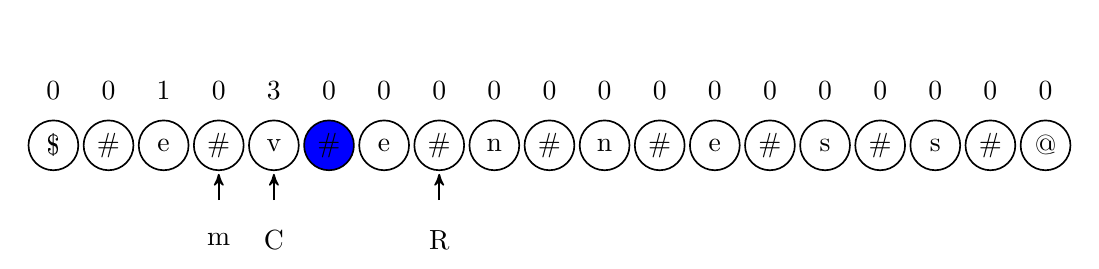
\begin{tikzpicture}[->,>=stealth',shorten >=1pt,auto,node distance=0.7cm,
                    semithick]
\tikzstyle{every state}=[fill=none,draw=black,text=black]
\tikzset{font=\fontsize{10pt}{12}\selectfont}

  
        \node[state,inner sep=2pt,minimum size=18pt]                (0)                           {\$};
        \node[state,inner sep=2pt,minimum size=18pt, draw=none]                (p0) [above of=0] {0};
        
        \node[state,inner sep=2pt,minimum size=18pt]                        (1)   [right of=0]          {\#};
        \node[state,inner sep=2pt,minimum size=18pt, draw=none]                (p1) [above of=1] {0};
        
        \node[state,inner sep=2pt,minimum size=18pt]                        (2)   [right of=1]          {e};
        \node[state,inner sep=2pt,minimum size=18pt, draw=none]                (p2) [above of=2] {1};
        
        \node[state,inner sep=2pt,minimum size=18pt]                        (3)   [right of=2]          {\#};
        \node[state,inner sep=2pt,minimum size=18pt, draw=none]                (p3) [above of=3] {0};
        
        \node[state,inner sep=2pt,minimum size=18pt]              (4)   [right of=3]          {v}; 
        \node[state,inner sep=2pt,minimum size=18pt, draw=none]                (p4) [above of=4] {3};
           
        \node[state,inner sep=2pt,minimum size=18pt, fill=blue]                        (5)   [right of=4]          {\#};
        \node[state,inner sep=2pt,minimum size=18pt, draw=none]                (p5) [above of=5] {0};
        
        \node[state,inner sep=2pt,minimum size=18pt]                        (6)   [right of=5]          {e};
        \node[state,inner sep=2pt,minimum size=18pt, draw=none]                (p6) [above of=6] {0};
        
        \node[state,inner sep=2pt,minimum size=18pt]                        (7)   [right of=6]          {\#};
        \node[state,inner sep=2pt,minimum size=18pt, draw=none]                (p7) [above of=7] {0};
        
        \node[state,inner sep=2pt,minimum size=18pt]              (8)   [right of=7]          {n};
        \node[state,inner sep=2pt,minimum size=18pt, draw=none]                (p8) [above of=8] {0};
            
        \node[state,inner sep=2pt,minimum size=18pt]                        (9)   [right of=8]          {\#};
        \node[state,inner sep=2pt,minimum size=18pt, draw=none]                (p9) [above of=9] {0};
        
        \node[state,inner sep=2pt,minimum size=18pt]                        (10)   [right of=9]          {n};
        \node[state,inner sep=2pt,minimum size=18pt, draw=none]                (p10) [above of=10] {0};
        
        \node[state,inner sep=2pt,minimum size=18pt]                        (11)   [right of=10]          {\#};
        \node[state,inner sep=2pt,minimum size=18pt, draw=none]                (p11) [above of=11] {0};
        
        \node[state,inner sep=2pt,minimum size=18pt]                        (12)   [right of=11]          {e};
        \node[state,inner sep=2pt,minimum size=18pt, draw=none]                (p12) [above of=12] {0};
        
        \node[state,inner sep=2pt,minimum size=18pt]                        (13)   [right of=12]          {\#};
        \node[state,inner sep=2pt,minimum size=18pt, draw=none]                (p13) [above of=13] {0};
        
        \node[state,inner sep=2pt,minimum size=18pt]              (14)   [right of=13]          {s};
        \node[state,inner sep=2pt,minimum size=18pt, draw=none]                (p14) [above of=14] {0};
            
        \node[state,inner sep=2pt,minimum size=18pt]                        (15)   [right of=14]          {\#};
        \node[state,inner sep=2pt,minimum size=18pt, draw=none]                (p15) [above of=15] {0};
        
        \node[state,inner sep=2pt,minimum size=18pt]                        (16)   [right of=15]          {s};
        \node[state,inner sep=2pt,minimum size=18pt, draw=none]                (p16) [above of=16] {0};
        
        \node[state,inner sep=2pt,minimum size=18pt]                        (17)   [right of=16]          {\#};
        \node[state,inner sep=2pt,minimum size=18pt, draw=none]                (p17) [above of=17] {0};
        
        \node[state,inner sep=2pt,minimum size=18pt]                        (18)   [right of=17]          {@};
        \node[state,inner sep=2pt,minimum size=18pt, draw=none]                (p18) [above of=18] {0};
        
        \node[state,inner sep=2pt,minimum size=28pt,draw=none, node distance = 1.2 cm]	     (C) [below of=4] {C};
        \node[state,inner sep=2pt,minimum size=28pt,draw=none, node distance = 1.2 cm]	     (R) [below of=7] {R};
        \node[state,inner sep=2pt,minimum size=28pt,draw=none, node distance = 1.2 cm]	     (m) [below of=3] {m};        
 
        \path[->]
        (C)   edge node {}            (4)  
        (R)   edge node {}            (7)
        (m)   edge node {}          (3) 
        ; %end path 
        
\end{tikzpicture} 

\\
\hline

%---------------------------------------------------------------------------------------------------------------------------------------%

6 &

~

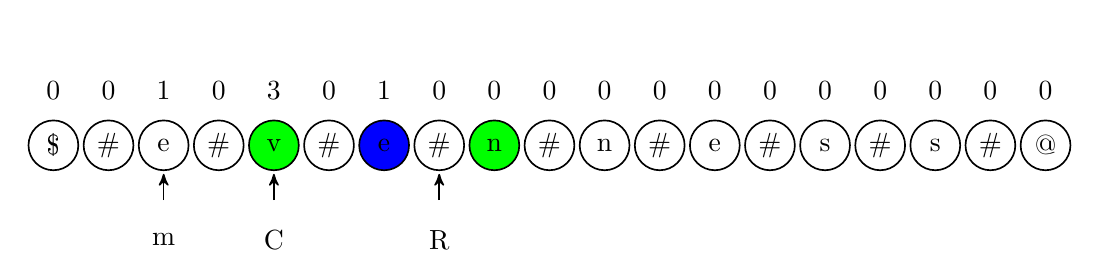
\begin{tikzpicture}[->,>=stealth',shorten >=1pt,auto,node distance=0.7cm,
                    semithick]
\tikzstyle{every state}=[fill=none,draw=black,text=black]
\tikzset{font=\fontsize{10pt}{12}\selectfont}

  
        \node[state,inner sep=2pt,minimum size=18pt]                (0)                           {\$};
        \node[state,inner sep=2pt,minimum size=18pt, draw=none]                (p0) [above of=0] {0};
        
        \node[state,inner sep=2pt,minimum size=18pt]                        (1)   [right of=0]          {\#};
        \node[state,inner sep=2pt,minimum size=18pt, draw=none]                (p1) [above of=1] {0};
        
        \node[state,inner sep=2pt,minimum size=18pt]                        (2)   [right of=1]          {e};
        \node[state,inner sep=2pt,minimum size=18pt, draw=none]                (p2) [above of=2] {1};
        
        \node[state,inner sep=2pt,minimum size=18pt]                        (3)   [right of=2]          {\#};
        \node[state,inner sep=2pt,minimum size=18pt, draw=none]                (p3) [above of=3] {0};
        
        \node[state,inner sep=2pt,minimum size=18pt, fill=green]              (4)   [right of=3]          {v}; 
        \node[state,inner sep=2pt,minimum size=18pt, draw=none]                (p4) [above of=4] {3};
           
        \node[state,inner sep=2pt,minimum size=18pt]                        (5)   [right of=4]          {\#};
        \node[state,inner sep=2pt,minimum size=18pt, draw=none]                (p5) [above of=5] {0};
        
        \node[state,inner sep=2pt,minimum size=18pt, fill=blue]                        (6)   [right of=5]          {e};
        \node[state,inner sep=2pt,minimum size=18pt, draw=none]                (p6) [above of=6] {1};
        
        \node[state,inner sep=2pt,minimum size=18pt]                        (7)   [right of=6]          {\#};
        \node[state,inner sep=2pt,minimum size=18pt, draw=none]                (p7) [above of=7] {0};
        
        \node[state,inner sep=2pt,minimum size=18pt, fill=green]              (8)   [right of=7]          {n};
        \node[state,inner sep=2pt,minimum size=18pt, draw=none]                (p8) [above of=8] {0};
            
        \node[state,inner sep=2pt,minimum size=18pt]                        (9)   [right of=8]          {\#};
        \node[state,inner sep=2pt,minimum size=18pt, draw=none]                (p9) [above of=9] {0};
        
        \node[state,inner sep=2pt,minimum size=18pt]                        (10)   [right of=9]          {n};
        \node[state,inner sep=2pt,minimum size=18pt, draw=none]                (p10) [above of=10] {0};
        
        \node[state,inner sep=2pt,minimum size=18pt]                        (11)   [right of=10]          {\#};
        \node[state,inner sep=2pt,minimum size=18pt, draw=none]                (p11) [above of=11] {0};
        
        \node[state,inner sep=2pt,minimum size=18pt]                        (12)   [right of=11]          {e};
        \node[state,inner sep=2pt,minimum size=18pt, draw=none]                (p12) [above of=12] {0};
        
        \node[state,inner sep=2pt,minimum size=18pt]                        (13)   [right of=12]          {\#};
        \node[state,inner sep=2pt,minimum size=18pt, draw=none]                (p13) [above of=13] {0};
        
        \node[state,inner sep=2pt,minimum size=18pt]              (14)   [right of=13]          {s};
        \node[state,inner sep=2pt,minimum size=18pt, draw=none]                (p14) [above of=14] {0};
            
        \node[state,inner sep=2pt,minimum size=18pt]                        (15)   [right of=14]          {\#};
        \node[state,inner sep=2pt,minimum size=18pt, draw=none]                (p15) [above of=15] {0};
        
        \node[state,inner sep=2pt,minimum size=18pt]                        (16)   [right of=15]          {s};
        \node[state,inner sep=2pt,minimum size=18pt, draw=none]                (p16) [above of=16] {0};
        
        \node[state,inner sep=2pt,minimum size=18pt]                        (17)   [right of=16]          {\#};
        \node[state,inner sep=2pt,minimum size=18pt, draw=none]                (p17) [above of=17] {0};
        
        \node[state,inner sep=2pt,minimum size=18pt]                        (18)   [right of=17]          {@};
        \node[state,inner sep=2pt,minimum size=18pt, draw=none]                (p18) [above of=18] {0};
        
        \node[state,inner sep=2pt,minimum size=28pt,draw=none, node distance = 1.2 cm]	     (C) [below of=4] {C};
        \node[state,inner sep=2pt,minimum size=28pt,draw=none, node distance = 1.2 cm]	     (R) [below of=7] {R};
        \node[state,inner sep=2pt,minimum size=28pt,draw=none, node distance = 1.2 cm]	     (m) [below of=2] {m};        
 
        \path[->]
        (C)   edge node {}            (4)  
        (R)   edge node {}            (7)
        (m)   edge node {}          (2) 
        ; %end path 
        
\end{tikzpicture} 

\\

\hline
\end{tabular}

%---------------------------------------------------------------------------------------------------------------------------------------%
\begin{tabular}{| c | p {14 cm} |}
\hline

7 &

~

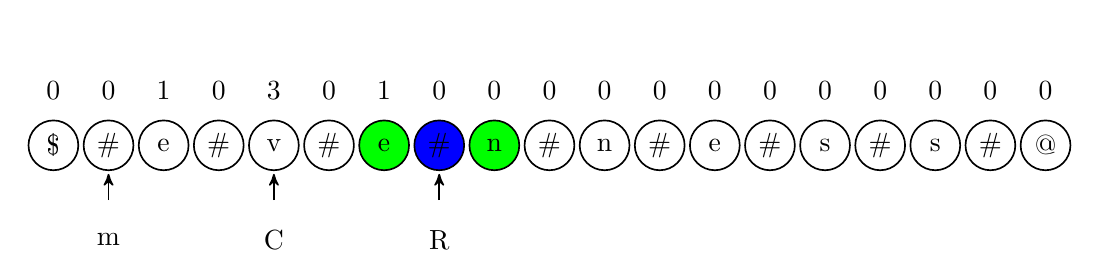
\begin{tikzpicture}[->,>=stealth',shorten >=1pt,auto,node distance=0.7cm,
                    semithick]
\tikzstyle{every state}=[fill=none,draw=black,text=black]
\tikzset{font=\fontsize{10pt}{12}\selectfont}

  
        \node[state,inner sep=2pt,minimum size=18pt]                (0)                           {\$};
        \node[state,inner sep=2pt,minimum size=18pt, draw=none]                (p0) [above of=0] {0};
        
        \node[state,inner sep=2pt,minimum size=18pt]                        (1)   [right of=0]          {\#};
        \node[state,inner sep=2pt,minimum size=18pt, draw=none]                (p1) [above of=1] {0};
        
        \node[state,inner sep=2pt,minimum size=18pt]                        (2)   [right of=1]          {e};
        \node[state,inner sep=2pt,minimum size=18pt, draw=none]                (p2) [above of=2] {1};
        
        \node[state,inner sep=2pt,minimum size=18pt]                        (3)   [right of=2]          {\#};
        \node[state,inner sep=2pt,minimum size=18pt, draw=none]                (p3) [above of=3] {0};
        
        \node[state,inner sep=2pt,minimum size=18pt]              (4)   [right of=3]          {v}; 
        \node[state,inner sep=2pt,minimum size=18pt, draw=none]                (p4) [above of=4] {3};
           
        \node[state,inner sep=2pt,minimum size=18pt]                        (5)   [right of=4]          {\#};
        \node[state,inner sep=2pt,minimum size=18pt, draw=none]                (p5) [above of=5] {0};
        
        \node[state,inner sep=2pt,minimum size=18pt, fill=green]                        (6)   [right of=5]          {e};
        \node[state,inner sep=2pt,minimum size=18pt, draw=none]                (p6) [above of=6] {1};
        
        \node[state,inner sep=2pt,minimum size=18pt, fill=blue]                        (7)   [right of=6]          {\#};
        \node[state,inner sep=2pt,minimum size=18pt, draw=none]                (p7) [above of=7] {0};
        
        \node[state,inner sep=2pt,minimum size=18pt, fill=green]              (8)   [right of=7]          {n};
        \node[state,inner sep=2pt,minimum size=18pt, draw=none]                (p8) [above of=8] {0};
            
        \node[state,inner sep=2pt,minimum size=18pt]                        (9)   [right of=8]          {\#};
        \node[state,inner sep=2pt,minimum size=18pt, draw=none]                (p9) [above of=9] {0};
        
        \node[state,inner sep=2pt,minimum size=18pt]                        (10)   [right of=9]          {n};
        \node[state,inner sep=2pt,minimum size=18pt, draw=none]                (p10) [above of=10] {0};
        
        \node[state,inner sep=2pt,minimum size=18pt]                        (11)   [right of=10]          {\#};
        \node[state,inner sep=2pt,minimum size=18pt, draw=none]                (p11) [above of=11] {0};
        
        \node[state,inner sep=2pt,minimum size=18pt]                        (12)   [right of=11]          {e};
        \node[state,inner sep=2pt,minimum size=18pt, draw=none]                (p12) [above of=12] {0};
        
        \node[state,inner sep=2pt,minimum size=18pt]                        (13)   [right of=12]          {\#};
        \node[state,inner sep=2pt,minimum size=18pt, draw=none]                (p13) [above of=13] {0};
        
        \node[state,inner sep=2pt,minimum size=18pt]              (14)   [right of=13]          {s};
        \node[state,inner sep=2pt,minimum size=18pt, draw=none]                (p14) [above of=14] {0};
            
        \node[state,inner sep=2pt,minimum size=18pt]                        (15)   [right of=14]          {\#};
        \node[state,inner sep=2pt,minimum size=18pt, draw=none]                (p15) [above of=15] {0};
        
        \node[state,inner sep=2pt,minimum size=18pt]                        (16)   [right of=15]          {s};
        \node[state,inner sep=2pt,minimum size=18pt, draw=none]                (p16) [above of=16] {0};
        
        \node[state,inner sep=2pt,minimum size=18pt]                        (17)   [right of=16]          {\#};
        \node[state,inner sep=2pt,minimum size=18pt, draw=none]                (p17) [above of=17] {0};
        
        \node[state,inner sep=2pt,minimum size=18pt]                        (18)   [right of=17]          {@};
        \node[state,inner sep=2pt,minimum size=18pt, draw=none]                (p18) [above of=18] {0};
        
        \node[state,inner sep=2pt,minimum size=28pt,draw=none, node distance = 1.2 cm]	     (C) [below of=4] {C};
        \node[state,inner sep=2pt,minimum size=28pt,draw=none, node distance = 1.2 cm]	     (R) [below of=7] {R};
        \node[state,inner sep=2pt,minimum size=28pt,draw=none, node distance = 1.2 cm]	     (m) [below of=1] {m};        
 
        \path[->]
        (C)   edge node {}            (4)  
        (R)   edge node {}            (7)
        (m)   edge node {}          (1) 
        ; %end path 
        
\end{tikzpicture} 

\\


%---------------------------------------------------------------------------------------------------------------------------------------%

\hline

8 &

~

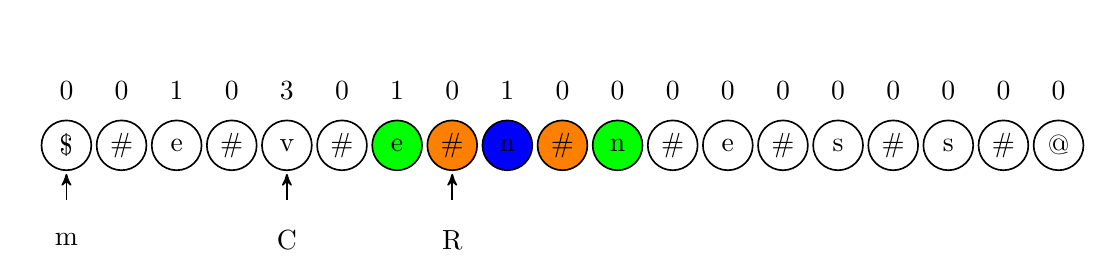
\begin{tikzpicture}[->,>=stealth',shorten >=1pt,auto,node distance=0.7cm,
                    semithick]
\tikzstyle{every state}=[fill=none,draw=black,text=black]
\tikzset{font=\fontsize{10pt}{12}\selectfont}

  
        \node[state,inner sep=2pt,minimum size=18pt]                (0)                           {\$};
        \node[state,inner sep=2pt,minimum size=18pt, draw=none]                (p0) [above of=0] {0};
        
        \node[state,inner sep=2pt,minimum size=18pt]                        (1)   [right of=0]          {\#};
        \node[state,inner sep=2pt,minimum size=18pt, draw=none]                (p1) [above of=1] {0};
        
        \node[state,inner sep=2pt,minimum size=18pt]                        (2)   [right of=1]          {e};
        \node[state,inner sep=2pt,minimum size=18pt, draw=none]                (p2) [above of=2] {1};
        
        \node[state,inner sep=2pt,minimum size=18pt]                        (3)   [right of=2]          {\#};
        \node[state,inner sep=2pt,minimum size=18pt, draw=none]                (p3) [above of=3] {0};
        
        \node[state,inner sep=2pt,minimum size=18pt]              (4)   [right of=3]          {v}; 
        \node[state,inner sep=2pt,minimum size=18pt, draw=none]                (p4) [above of=4] {3};
           
        \node[state,inner sep=2pt,minimum size=18pt]                        (5)   [right of=4]          {\#};
        \node[state,inner sep=2pt,minimum size=18pt, draw=none]                (p5) [above of=5] {0};
        
        \node[state,inner sep=2pt,minimum size=18pt, fill=green]                        (6)   [right of=5]          {e};
        \node[state,inner sep=2pt,minimum size=18pt, draw=none]                (p6) [above of=6] {1};
        
        \node[state,inner sep=2pt,minimum size=18pt, fill=orange]                        (7)   [right of=6]          {\#};
        \node[state,inner sep=2pt,minimum size=18pt, draw=none]                (p7) [above of=7] {0};
        
        \node[state,inner sep=2pt,minimum size=18pt, fill=blue]              (8)   [right of=7]          {n};
        \node[state,inner sep=2pt,minimum size=18pt, draw=none]                (p8) [above of=8] {1};
            
        \node[state,inner sep=2pt,minimum size=18pt, fill=orange]                        (9)   [right of=8]          {\#};
        \node[state,inner sep=2pt,minimum size=18pt, draw=none]                (p9) [above of=9] {0};
        
        \node[state,inner sep=2pt,minimum size=18pt, fill=green]                        (10)   [right of=9]          {n};
        \node[state,inner sep=2pt,minimum size=18pt, draw=none]                (p10) [above of=10] {0};
        
        \node[state,inner sep=2pt,minimum size=18pt]                        (11)   [right of=10]          {\#};
        \node[state,inner sep=2pt,minimum size=18pt, draw=none]                (p11) [above of=11] {0};
        
        \node[state,inner sep=2pt,minimum size=18pt]                        (12)   [right of=11]          {e};
        \node[state,inner sep=2pt,minimum size=18pt, draw=none]                (p12) [above of=12] {0};
        
        \node[state,inner sep=2pt,minimum size=18pt]                        (13)   [right of=12]          {\#};
        \node[state,inner sep=2pt,minimum size=18pt, draw=none]                (p13) [above of=13] {0};
        
        \node[state,inner sep=2pt,minimum size=18pt]              (14)   [right of=13]          {s};
        \node[state,inner sep=2pt,minimum size=18pt, draw=none]                (p14) [above of=14] {0};
            
        \node[state,inner sep=2pt,minimum size=18pt]                        (15)   [right of=14]          {\#};
        \node[state,inner sep=2pt,minimum size=18pt, draw=none]                (p15) [above of=15] {0};
        
        \node[state,inner sep=2pt,minimum size=18pt]                        (16)   [right of=15]          {s};
        \node[state,inner sep=2pt,minimum size=18pt, draw=none]                (p16) [above of=16] {0};
        
        \node[state,inner sep=2pt,minimum size=18pt]                        (17)   [right of=16]          {\#};
        \node[state,inner sep=2pt,minimum size=18pt, draw=none]                (p17) [above of=17] {0};
        
        \node[state,inner sep=2pt,minimum size=18pt]                        (18)   [right of=17]          {@};
        \node[state,inner sep=2pt,minimum size=18pt, draw=none]                (p18) [above of=18] {0};
        
        \node[state,inner sep=2pt,minimum size=28pt,draw=none, node distance = 1.2 cm]	     (C) [below of=4] {C};
        \node[state,inner sep=2pt,minimum size=28pt,draw=none, node distance = 1.2 cm]	     (R) [below of=7] {R};
        \node[state,inner sep=2pt,minimum size=28pt,draw=none, node distance = 1.2 cm]	     (m) [below of=0] {m};        
 
        \path[->]
        (C)   edge node {}            (4)  
        (R)   edge node {}            (7)
        (m)   edge node {}          (0) 
        ; %end path 
        
\end{tikzpicture} 

\\
%---------------------------------------------------------------------------------------------------------------------------------------%
\hline

9 &

~

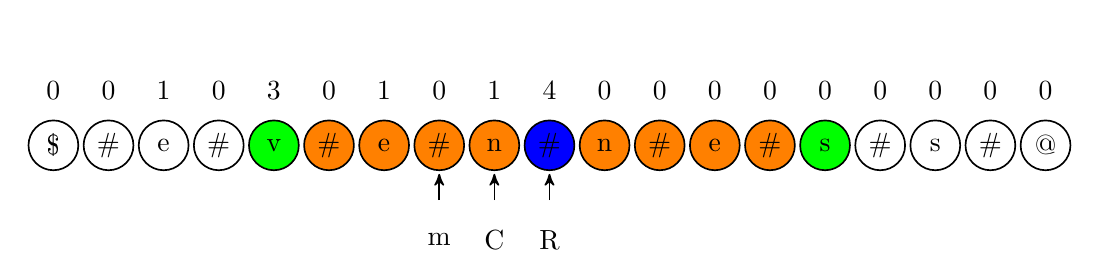
\begin{tikzpicture}[->,>=stealth',shorten >=1pt,auto,node distance=0.7cm,
                    semithick]
\tikzstyle{every state}=[fill=none,draw=black,text=black]
\tikzset{font=\fontsize{10pt}{12}\selectfont}

  
        \node[state,inner sep=2pt,minimum size=18pt]                (0)                           {\$};
        \node[state,inner sep=2pt,minimum size=18pt, draw=none]                (p0) [above of=0] {0};
        
        \node[state,inner sep=2pt,minimum size=18pt]                        (1)   [right of=0]          {\#};
        \node[state,inner sep=2pt,minimum size=18pt, draw=none]                (p1) [above of=1] {0};
        
        \node[state,inner sep=2pt,minimum size=18pt]                        (2)   [right of=1]          {e};
        \node[state,inner sep=2pt,minimum size=18pt, draw=none]                (p2) [above of=2] {1};
        
        \node[state,inner sep=2pt,minimum size=18pt]                        (3)   [right of=2]          {\#};
        \node[state,inner sep=2pt,minimum size=18pt, draw=none]                (p3) [above of=3] {0};
        
        \node[state,inner sep=2pt,minimum size=18pt, fill=green]              (4)   [right of=3]          {v}; 
        \node[state,inner sep=2pt,minimum size=18pt, draw=none]                (p4) [above of=4] {3};
           
        \node[state,inner sep=2pt,minimum size=18pt, fill=orange]                        (5)   [right of=4]          {\#};
        \node[state,inner sep=2pt,minimum size=18pt, draw=none]                (p5) [above of=5] {0};
        
        \node[state,inner sep=2pt,minimum size=18pt, fill=orange]                        (6)   [right of=5]          {e};
        \node[state,inner sep=2pt,minimum size=18pt, draw=none]                (p6) [above of=6] {1};
        
        \node[state,inner sep=2pt,minimum size=18pt, fill=orange]                        (7)   [right of=6]          {\#};
        \node[state,inner sep=2pt,minimum size=18pt, draw=none]                (p7) [above of=7] {0};
        
        \node[state,inner sep=2pt,minimum size=18pt, fill=orange]              (8)   [right of=7]          {n};
        \node[state,inner sep=2pt,minimum size=18pt, draw=none]                (p8) [above of=8] {1};
            
        \node[state,inner sep=2pt,minimum size=18pt, fill=blue]                        (9)   [right of=8]          {\#};
        \node[state,inner sep=2pt,minimum size=18pt, draw=none]                (p9) [above of=9] {4};
        
        \node[state,inner sep=2pt,minimum size=18pt, fill=orange]                        (10)   [right of=9]          {n};
        \node[state,inner sep=2pt,minimum size=18pt, draw=none]                (p10) [above of=10] {0};
        
        \node[state,inner sep=2pt,minimum size=18pt, fill=orange]                        (11)   [right of=10]          {\#};
        \node[state,inner sep=2pt,minimum size=18pt, draw=none]                (p11) [above of=11] {0};
        
        \node[state,inner sep=2pt,minimum size=18pt, fill=orange]                        (12)   [right of=11]          {e};
        \node[state,inner sep=2pt,minimum size=18pt, draw=none]                (p12) [above of=12] {0};
        
        \node[state,inner sep=2pt,minimum size=18pt, fill=orange]                        (13)   [right of=12]          {\#};
        \node[state,inner sep=2pt,minimum size=18pt, draw=none]                (p13) [above of=13] {0};
        
        \node[state,inner sep=2pt,minimum size=18pt, fill=green]              (14)   [right of=13]          {s};
        \node[state,inner sep=2pt,minimum size=18pt, draw=none]                (p14) [above of=14] {0};
            
        \node[state,inner sep=2pt,minimum size=18pt]                        (15)   [right of=14]          {\#};
        \node[state,inner sep=2pt,minimum size=18pt, draw=none]                (p15) [above of=15] {0};
        
        \node[state,inner sep=2pt,minimum size=18pt]                        (16)   [right of=15]          {s};
        \node[state,inner sep=2pt,minimum size=18pt, draw=none]                (p16) [above of=16] {0};
        
        \node[state,inner sep=2pt,minimum size=18pt]                        (17)   [right of=16]          {\#};
        \node[state,inner sep=2pt,minimum size=18pt, draw=none]                (p17) [above of=17] {0};
        
        \node[state,inner sep=2pt,minimum size=18pt]                        (18)   [right of=17]          {@};
        \node[state,inner sep=2pt,minimum size=18pt, draw=none]                (p18) [above of=18] {0};
        
        \node[state,inner sep=2pt,minimum size=28pt,draw=none, node distance = 1.2 cm]	     (C) [below of=8] {C};
        \node[state,inner sep=2pt,minimum size=28pt,draw=none, node distance = 1.2 cm]	     (R) [below of=9] {R};
        \node[state,inner sep=2pt,minimum size=28pt,draw=none, node distance = 1.2 cm]	     (m) [below of=7] {m};        
 
        \path[->]
        (C)   edge node {}            (8)  
        (R)   edge node {}            (9)
        (m)   edge node {}          (7) 
        ; %end path 
        
\end{tikzpicture} 

\\
%---------------------------------------------------------------------------------------------------------------------------------------%
\hline

10 &

~

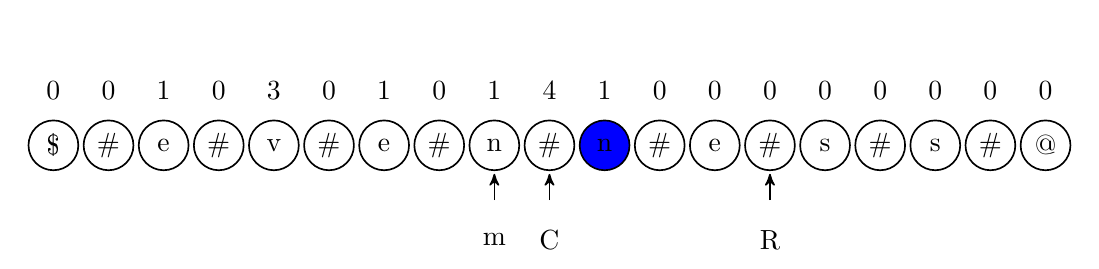
\begin{tikzpicture}[->,>=stealth',shorten >=1pt,auto,node distance=0.7cm,
                    semithick]
\tikzstyle{every state}=[fill=none,draw=black,text=black]
\tikzset{font=\fontsize{10pt}{12}\selectfont}

  
        \node[state,inner sep=2pt,minimum size=18pt]                (0)                           {\$};
        \node[state,inner sep=2pt,minimum size=18pt, draw=none]                (p0) [above of=0] {0};
        
        \node[state,inner sep=2pt,minimum size=18pt]                        (1)   [right of=0]          {\#};
        \node[state,inner sep=2pt,minimum size=18pt, draw=none]                (p1) [above of=1] {0};
        
        \node[state,inner sep=2pt,minimum size=18pt]                        (2)   [right of=1]          {e};
        \node[state,inner sep=2pt,minimum size=18pt, draw=none]                (p2) [above of=2] {1};
        
        \node[state,inner sep=2pt,minimum size=18pt]                        (3)   [right of=2]          {\#};
        \node[state,inner sep=2pt,minimum size=18pt, draw=none]                (p3) [above of=3] {0};
        
        \node[state,inner sep=2pt,minimum size=18pt]              (4)   [right of=3]          {v}; 
        \node[state,inner sep=2pt,minimum size=18pt, draw=none]                (p4) [above of=4] {3};
           
        \node[state,inner sep=2pt,minimum size=18pt]                        (5)   [right of=4]          {\#};
        \node[state,inner sep=2pt,minimum size=18pt, draw=none]                (p5) [above of=5] {0};
        
        \node[state,inner sep=2pt,minimum size=18pt]                        (6)   [right of=5]          {e};
        \node[state,inner sep=2pt,minimum size=18pt, draw=none]                (p6) [above of=6] {1};
        
        \node[state,inner sep=2pt,minimum size=18pt]                        (7)   [right of=6]          {\#};
        \node[state,inner sep=2pt,minimum size=18pt, draw=none]                (p7) [above of=7] {0};
        
        \node[state,inner sep=2pt,minimum size=18pt]              (8)   [right of=7]          {n};
        \node[state,inner sep=2pt,minimum size=18pt, draw=none]                (p8) [above of=8] {1};
            
        \node[state,inner sep=2pt,minimum size=18pt]                        (9)   [right of=8]          {\#};
        \node[state,inner sep=2pt,minimum size=18pt, draw=none]                (p9) [above of=9] {4};
        
        \node[state,inner sep=2pt,minimum size=18pt, fill=blue]                        (10)   [right of=9]          {n};
        \node[state,inner sep=2pt,minimum size=18pt, draw=none]                (p10) [above of=10] {1};
        
        \node[state,inner sep=2pt,minimum size=18pt]                        (11)   [right of=10]          {\#};
        \node[state,inner sep=2pt,minimum size=18pt, draw=none]                (p11) [above of=11] {0};
        
        \node[state,inner sep=2pt,minimum size=18pt]                        (12)   [right of=11]          {e};
        \node[state,inner sep=2pt,minimum size=18pt, draw=none]                (p12) [above of=12] {0};
        
        \node[state,inner sep=2pt,minimum size=18pt]                        (13)   [right of=12]          {\#};
        \node[state,inner sep=2pt,minimum size=18pt, draw=none]                (p13) [above of=13] {0};
        
        \node[state,inner sep=2pt,minimum size=18pt]              (14)   [right of=13]          {s};
        \node[state,inner sep=2pt,minimum size=18pt, draw=none]                (p14) [above of=14] {0};
            
        \node[state,inner sep=2pt,minimum size=18pt]                        (15)   [right of=14]          {\#};
        \node[state,inner sep=2pt,minimum size=18pt, draw=none]                (p15) [above of=15] {0};
        
        \node[state,inner sep=2pt,minimum size=18pt]                        (16)   [right of=15]          {s};
        \node[state,inner sep=2pt,minimum size=18pt, draw=none]                (p16) [above of=16] {0};
        
        \node[state,inner sep=2pt,minimum size=18pt]                        (17)   [right of=16]          {\#};
        \node[state,inner sep=2pt,minimum size=18pt, draw=none]                (p17) [above of=17] {0};
        
        \node[state,inner sep=2pt,minimum size=18pt]                        (18)   [right of=17]          {@};
        \node[state,inner sep=2pt,minimum size=18pt, draw=none]                (p18) [above of=18] {0};
        
        \node[state,inner sep=2pt,minimum size=28pt,draw=none, node distance = 1.2 cm]	     (C) [below of=9] {C};
        \node[state,inner sep=2pt,minimum size=28pt,draw=none, node distance = 1.2 cm]	     (R) [below of=13] {R};
        \node[state,inner sep=2pt,minimum size=28pt,draw=none, node distance = 1.2 cm]	     (m) [below of=8] {m};        
 
        \path[->]
        (C)   edge node {}            (9)  
        (R)   edge node {}            (13)
        (m)   edge node {}          (8) 
        ; %end path 
        
\end{tikzpicture} 

\\
%---------------------------------------------------------------------------------------------------------------------------------------%
\hline

11 &

~

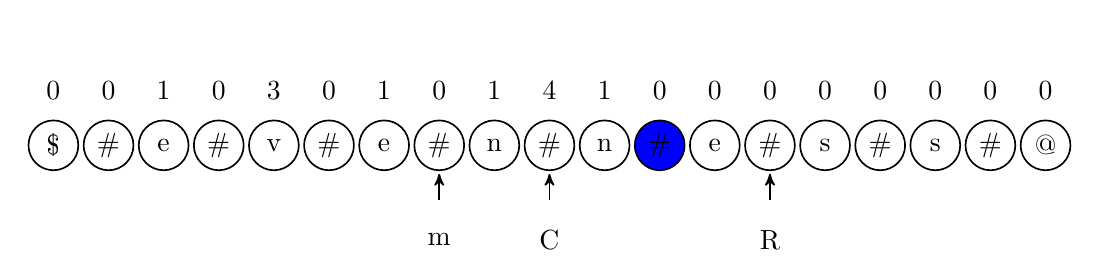
\begin{tikzpicture}[->,>=stealth',shorten >=1pt,auto,node distance=0.7cm,
                    semithick]
\tikzstyle{every state}=[fill=none,draw=black,text=black]
\tikzset{font=\fontsize{10pt}{12}\selectfont}

  
        \node[state,inner sep=2pt,minimum size=18pt]                (0)                           {\$};
        \node[state,inner sep=2pt,minimum size=18pt, draw=none]                (p0) [above of=0] {0};
        
        \node[state,inner sep=2pt,minimum size=18pt]                        (1)   [right of=0]          {\#};
        \node[state,inner sep=2pt,minimum size=18pt, draw=none]                (p1) [above of=1] {0};
        
        \node[state,inner sep=2pt,minimum size=18pt]                        (2)   [right of=1]          {e};
        \node[state,inner sep=2pt,minimum size=18pt, draw=none]                (p2) [above of=2] {1};
        
        \node[state,inner sep=2pt,minimum size=18pt]                        (3)   [right of=2]          {\#};
        \node[state,inner sep=2pt,minimum size=18pt, draw=none]                (p3) [above of=3] {0};
        
        \node[state,inner sep=2pt,minimum size=18pt]              (4)   [right of=3]          {v}; 
        \node[state,inner sep=2pt,minimum size=18pt, draw=none]                (p4) [above of=4] {3};
           
        \node[state,inner sep=2pt,minimum size=18pt]                        (5)   [right of=4]          {\#};
        \node[state,inner sep=2pt,minimum size=18pt, draw=none]                (p5) [above of=5] {0};
        
        \node[state,inner sep=2pt,minimum size=18pt]                        (6)   [right of=5]          {e};
        \node[state,inner sep=2pt,minimum size=18pt, draw=none]                (p6) [above of=6] {1};
        
        \node[state,inner sep=2pt,minimum size=18pt]                        (7)   [right of=6]          {\#};
        \node[state,inner sep=2pt,minimum size=18pt, draw=none]                (p7) [above of=7] {0};
        
        \node[state,inner sep=2pt,minimum size=18pt]              (8)   [right of=7]          {n};
        \node[state,inner sep=2pt,minimum size=18pt, draw=none]                (p8) [above of=8] {1};
            
        \node[state,inner sep=2pt,minimum size=18pt]                        (9)   [right of=8]          {\#};
        \node[state,inner sep=2pt,minimum size=18pt, draw=none]                (p9) [above of=9] {4};
        
        \node[state,inner sep=2pt,minimum size=18pt]                        (10)   [right of=9]          {n};
        \node[state,inner sep=2pt,minimum size=18pt, draw=none]                (p10) [above of=10] {1};
        
        \node[state,inner sep=2pt,minimum size=18pt, fill=blue]                        (11)   [right of=10]          {\#};
        \node[state,inner sep=2pt,minimum size=18pt, draw=none]                (p11) [above of=11] {0};
        
        \node[state,inner sep=2pt,minimum size=18pt]                        (12)   [right of=11]          {e};
        \node[state,inner sep=2pt,minimum size=18pt, draw=none]                (p12) [above of=12] {0};
        
        \node[state,inner sep=2pt,minimum size=18pt]                        (13)   [right of=12]          {\#};
        \node[state,inner sep=2pt,minimum size=18pt, draw=none]                (p13) [above of=13] {0};
        
        \node[state,inner sep=2pt,minimum size=18pt]              (14)   [right of=13]          {s};
        \node[state,inner sep=2pt,minimum size=18pt, draw=none]                (p14) [above of=14] {0};
            
        \node[state,inner sep=2pt,minimum size=18pt]                        (15)   [right of=14]          {\#};
        \node[state,inner sep=2pt,minimum size=18pt, draw=none]                (p15) [above of=15] {0};
        
        \node[state,inner sep=2pt,minimum size=18pt]                        (16)   [right of=15]          {s};
        \node[state,inner sep=2pt,minimum size=18pt, draw=none]                (p16) [above of=16] {0};
        
        \node[state,inner sep=2pt,minimum size=18pt]                        (17)   [right of=16]          {\#};
        \node[state,inner sep=2pt,minimum size=18pt, draw=none]                (p17) [above of=17] {0};
        
        \node[state,inner sep=2pt,minimum size=18pt]                        (18)   [right of=17]          {@};
        \node[state,inner sep=2pt,minimum size=18pt, draw=none]                (p18) [above of=18] {0};
        
        \node[state,inner sep=2pt,minimum size=28pt,draw=none, node distance = 1.2 cm]	     (C) [below of=9] {C};
        \node[state,inner sep=2pt,minimum size=28pt,draw=none, node distance = 1.2 cm]	     (R) [below of=13] {R};
        \node[state,inner sep=2pt,minimum size=28pt,draw=none, node distance = 1.2 cm]	     (m) [below of=7] {m};        
 
        \path[->]
        (C)   edge node {}            (9)  
        (R)   edge node {}            (13)
        (m)   edge node {}          (7) 
        ; %end path 
        
\end{tikzpicture} 

\\
%---------------------------------------------------------------------------------------------------------------------------------------%
\hline

12 &

~

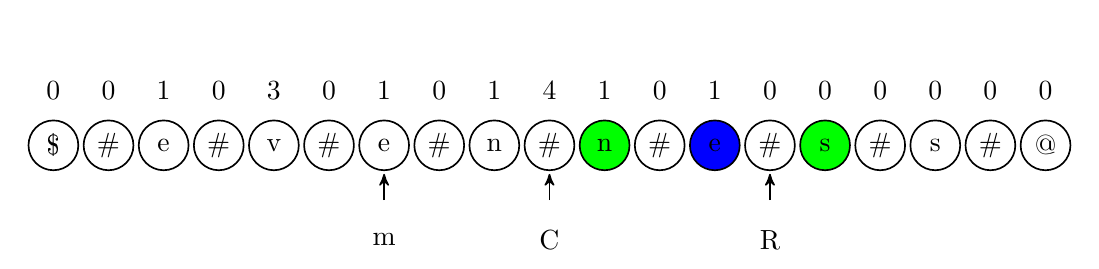
\begin{tikzpicture}[->,>=stealth',shorten >=1pt,auto,node distance=0.7cm,
                    semithick]
\tikzstyle{every state}=[fill=none,draw=black,text=black]
\tikzset{font=\fontsize{10pt}{12}\selectfont}

  
        \node[state,inner sep=2pt,minimum size=18pt]                (0)                           {\$};
        \node[state,inner sep=2pt,minimum size=18pt, draw=none]                (p0) [above of=0] {0};
        
        \node[state,inner sep=2pt,minimum size=18pt]                        (1)   [right of=0]          {\#};
        \node[state,inner sep=2pt,minimum size=18pt, draw=none]                (p1) [above of=1] {0};
        
        \node[state,inner sep=2pt,minimum size=18pt]                        (2)   [right of=1]          {e};
        \node[state,inner sep=2pt,minimum size=18pt, draw=none]                (p2) [above of=2] {1};
        
        \node[state,inner sep=2pt,minimum size=18pt]                        (3)   [right of=2]          {\#};
        \node[state,inner sep=2pt,minimum size=18pt, draw=none]                (p3) [above of=3] {0};
        
        \node[state,inner sep=2pt,minimum size=18pt]              (4)   [right of=3]          {v}; 
        \node[state,inner sep=2pt,minimum size=18pt, draw=none]                (p4) [above of=4] {3};
           
        \node[state,inner sep=2pt,minimum size=18pt]                        (5)   [right of=4]          {\#};
        \node[state,inner sep=2pt,minimum size=18pt, draw=none]                (p5) [above of=5] {0};
        
        \node[state,inner sep=2pt,minimum size=18pt]                        (6)   [right of=5]          {e};
        \node[state,inner sep=2pt,minimum size=18pt, draw=none]                (p6) [above of=6] {1};
        
        \node[state,inner sep=2pt,minimum size=18pt]                        (7)   [right of=6]          {\#};
        \node[state,inner sep=2pt,minimum size=18pt, draw=none]                (p7) [above of=7] {0};
        
        \node[state,inner sep=2pt,minimum size=18pt]              (8)   [right of=7]          {n};
        \node[state,inner sep=2pt,minimum size=18pt, draw=none]                (p8) [above of=8] {1};
            
        \node[state,inner sep=2pt,minimum size=18pt]                        (9)   [right of=8]          {\#};
        \node[state,inner sep=2pt,minimum size=18pt, draw=none]                (p9) [above of=9] {4};
        
        \node[state,inner sep=2pt,minimum size=18pt, fill=green]                        (10)   [right of=9]          {n};
        \node[state,inner sep=2pt,minimum size=18pt, draw=none]                (p10) [above of=10] {1};
        
        \node[state,inner sep=2pt,minimum size=18pt]                        (11)   [right of=10]          {\#};
        \node[state,inner sep=2pt,minimum size=18pt, draw=none]                (p11) [above of=11] {0};
        
        \node[state,inner sep=2pt,minimum size=18pt, fill=blue]                        (12)   [right of=11]          {e};
        \node[state,inner sep=2pt,minimum size=18pt, draw=none]                (p12) [above of=12] {1};
        
        \node[state,inner sep=2pt,minimum size=18pt]                        (13)   [right of=12]          {\#};
        \node[state,inner sep=2pt,minimum size=18pt, draw=none]                (p13) [above of=13] {0};
        
        \node[state,inner sep=2pt,minimum size=18pt, fill=green]              (14)   [right of=13]          {s};
        \node[state,inner sep=2pt,minimum size=18pt, draw=none]                (p14) [above of=14] {0};
            
        \node[state,inner sep=2pt,minimum size=18pt]                        (15)   [right of=14]          {\#};
        \node[state,inner sep=2pt,minimum size=18pt, draw=none]                (p15) [above of=15] {0};
        
        \node[state,inner sep=2pt,minimum size=18pt]                        (16)   [right of=15]          {s};
        \node[state,inner sep=2pt,minimum size=18pt, draw=none]                (p16) [above of=16] {0};
        
        \node[state,inner sep=2pt,minimum size=18pt]                        (17)   [right of=16]          {\#};
        \node[state,inner sep=2pt,minimum size=18pt, draw=none]                (p17) [above of=17] {0};
        
        \node[state,inner sep=2pt,minimum size=18pt]                        (18)   [right of=17]          {@};
        \node[state,inner sep=2pt,minimum size=18pt, draw=none]                (p18) [above of=18] {0};
        
        \node[state,inner sep=2pt,minimum size=28pt,draw=none, node distance = 1.2 cm]	     (C) [below of=9] {C};
        \node[state,inner sep=2pt,minimum size=28pt,draw=none, node distance = 1.2 cm]	     (R) [below of=13] {R};
        \node[state,inner sep=2pt,minimum size=28pt,draw=none, node distance = 1.2 cm]	     (m) [below of=6] {m};        
 
        \path[->]
        (C)   edge node {}            (9)  
        (R)   edge node {}            (13)
        (m)   edge node {}          (6) 
        ; %end path 
        
\end{tikzpicture} 

\\
\hline
\end{tabular}
%---------------------------------------------------------------------------------------------------------------------------------------%
\begin{tabular}{| c | p {14 cm} |}

\hline

13 &

~

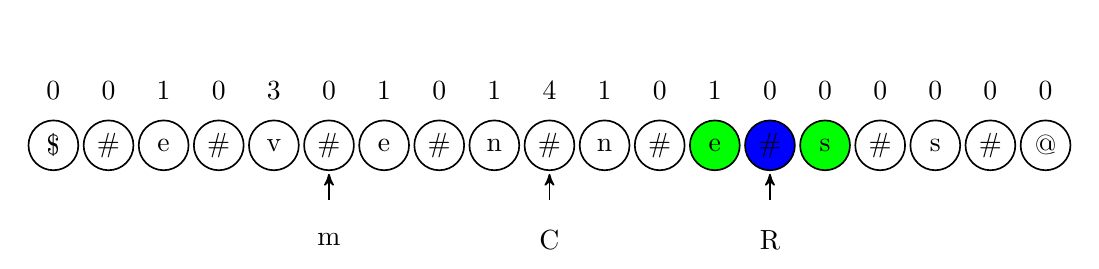
\begin{tikzpicture}[->,>=stealth',shorten >=1pt,auto,node distance=0.7cm,
                    semithick]
\tikzstyle{every state}=[fill=none,draw=black,text=black]
\tikzset{font=\fontsize{10pt}{12}\selectfont}

  
        \node[state,inner sep=2pt,minimum size=18pt]                (0)                           {\$};
        \node[state,inner sep=2pt,minimum size=18pt, draw=none]                (p0) [above of=0] {0};
        
        \node[state,inner sep=2pt,minimum size=18pt]                        (1)   [right of=0]          {\#};
        \node[state,inner sep=2pt,minimum size=18pt, draw=none]                (p1) [above of=1] {0};
        
        \node[state,inner sep=2pt,minimum size=18pt]                        (2)   [right of=1]          {e};
        \node[state,inner sep=2pt,minimum size=18pt, draw=none]                (p2) [above of=2] {1};
        
        \node[state,inner sep=2pt,minimum size=18pt]                        (3)   [right of=2]          {\#};
        \node[state,inner sep=2pt,minimum size=18pt, draw=none]                (p3) [above of=3] {0};
        
        \node[state,inner sep=2pt,minimum size=18pt]              (4)   [right of=3]          {v}; 
        \node[state,inner sep=2pt,minimum size=18pt, draw=none]                (p4) [above of=4] {3};
           
        \node[state,inner sep=2pt,minimum size=18pt]                        (5)   [right of=4]          {\#};
        \node[state,inner sep=2pt,minimum size=18pt, draw=none]                (p5) [above of=5] {0};
        
        \node[state,inner sep=2pt,minimum size=18pt]                        (6)   [right of=5]          {e};
        \node[state,inner sep=2pt,minimum size=18pt, draw=none]                (p6) [above of=6] {1};
        
        \node[state,inner sep=2pt,minimum size=18pt]                        (7)   [right of=6]          {\#};
        \node[state,inner sep=2pt,minimum size=18pt, draw=none]                (p7) [above of=7] {0};
        
        \node[state,inner sep=2pt,minimum size=18pt]              (8)   [right of=7]          {n};
        \node[state,inner sep=2pt,minimum size=18pt, draw=none]                (p8) [above of=8] {1};
            
        \node[state,inner sep=2pt,minimum size=18pt]                        (9)   [right of=8]          {\#};
        \node[state,inner sep=2pt,minimum size=18pt, draw=none]                (p9) [above of=9] {4};
        
        \node[state,inner sep=2pt,minimum size=18pt]                        (10)   [right of=9]          {n};
        \node[state,inner sep=2pt,minimum size=18pt, draw=none]                (p10) [above of=10] {1};
        
        \node[state,inner sep=2pt,minimum size=18pt]                        (11)   [right of=10]          {\#};
        \node[state,inner sep=2pt,minimum size=18pt, draw=none]                (p11) [above of=11] {0};
        
        \node[state,inner sep=2pt,minimum size=18pt, fill=green]                        (12)   [right of=11]          {e};
        \node[state,inner sep=2pt,minimum size=18pt, draw=none]                (p12) [above of=12] {1};
        
        \node[state,inner sep=2pt,minimum size=18pt, fill=blue]                        (13)   [right of=12]          {\#};
        \node[state,inner sep=2pt,minimum size=18pt, draw=none]                (p13) [above of=13] {0};
        
        \node[state,inner sep=2pt,minimum size=18pt, fill=green]              (14)   [right of=13]          {s};
        \node[state,inner sep=2pt,minimum size=18pt, draw=none]                (p14) [above of=14] {0};
            
        \node[state,inner sep=2pt,minimum size=18pt]                        (15)   [right of=14]          {\#};
        \node[state,inner sep=2pt,minimum size=18pt, draw=none]                (p15) [above of=15] {0};
        
        \node[state,inner sep=2pt,minimum size=18pt]                        (16)   [right of=15]          {s};
        \node[state,inner sep=2pt,minimum size=18pt, draw=none]                (p16) [above of=16] {0};
        
        \node[state,inner sep=2pt,minimum size=18pt]                        (17)   [right of=16]          {\#};
        \node[state,inner sep=2pt,minimum size=18pt, draw=none]                (p17) [above of=17] {0};
        
        \node[state,inner sep=2pt,minimum size=18pt]                        (18)   [right of=17]          {@};
        \node[state,inner sep=2pt,minimum size=18pt, draw=none]                (p18) [above of=18] {0};
        
        \node[state,inner sep=2pt,minimum size=28pt,draw=none, node distance = 1.2 cm]	     (C) [below of=9] {C};
        \node[state,inner sep=2pt,minimum size=28pt,draw=none, node distance = 1.2 cm]	     (R) [below of=13] {R};
        \node[state,inner sep=2pt,minimum size=28pt,draw=none, node distance = 1.2 cm]	     (m) [below of=5] {m};        
 
        \path[->]
        (C)   edge node {}            (9)  
        (R)   edge node {}            (13)
        (m)   edge node {}          (5) 
        ; %end path 
        
\end{tikzpicture} 

\\
%---------------------------------------------------------------------------------------------------------------------------------------%
\hline

14 &

~

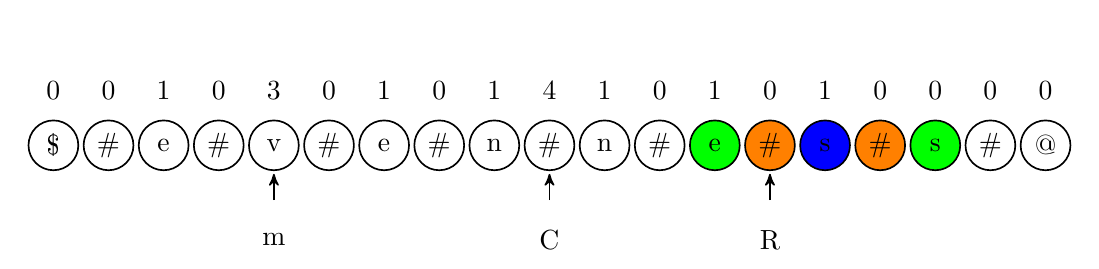
\begin{tikzpicture}[->,>=stealth',shorten >=1pt,auto,node distance=0.7cm,
                    semithick]
\tikzstyle{every state}=[fill=none,draw=black,text=black]
\tikzset{font=\fontsize{10pt}{12}\selectfont}

  
        \node[state,inner sep=2pt,minimum size=18pt]                (0)                           {\$};
        \node[state,inner sep=2pt,minimum size=18pt, draw=none]                (p0) [above of=0] {0};
        
        \node[state,inner sep=2pt,minimum size=18pt]                        (1)   [right of=0]          {\#};
        \node[state,inner sep=2pt,minimum size=18pt, draw=none]                (p1) [above of=1] {0};
        
        \node[state,inner sep=2pt,minimum size=18pt]                        (2)   [right of=1]          {e};
        \node[state,inner sep=2pt,minimum size=18pt, draw=none]                (p2) [above of=2] {1};
        
        \node[state,inner sep=2pt,minimum size=18pt]                        (3)   [right of=2]          {\#};
        \node[state,inner sep=2pt,minimum size=18pt, draw=none]                (p3) [above of=3] {0};
        
        \node[state,inner sep=2pt,minimum size=18pt]              (4)   [right of=3]          {v}; 
        \node[state,inner sep=2pt,minimum size=18pt, draw=none]                (p4) [above of=4] {3};
           
        \node[state,inner sep=2pt,minimum size=18pt]                        (5)   [right of=4]          {\#};
        \node[state,inner sep=2pt,minimum size=18pt, draw=none]                (p5) [above of=5] {0};
        
        \node[state,inner sep=2pt,minimum size=18pt]                        (6)   [right of=5]          {e};
        \node[state,inner sep=2pt,minimum size=18pt, draw=none]                (p6) [above of=6] {1};
        
        \node[state,inner sep=2pt,minimum size=18pt]                        (7)   [right of=6]          {\#};
        \node[state,inner sep=2pt,minimum size=18pt, draw=none]                (p7) [above of=7] {0};
        
        \node[state,inner sep=2pt,minimum size=18pt]              (8)   [right of=7]          {n};
        \node[state,inner sep=2pt,minimum size=18pt, draw=none]                (p8) [above of=8] {1};
            
        \node[state,inner sep=2pt,minimum size=18pt]                        (9)   [right of=8]          {\#};
        \node[state,inner sep=2pt,minimum size=18pt, draw=none]                (p9) [above of=9] {4};
        
        \node[state,inner sep=2pt,minimum size=18pt]                        (10)   [right of=9]          {n};
        \node[state,inner sep=2pt,minimum size=18pt, draw=none]                (p10) [above of=10] {1};
        
        \node[state,inner sep=2pt,minimum size=18pt]                        (11)   [right of=10]          {\#};
        \node[state,inner sep=2pt,minimum size=18pt, draw=none]                (p11) [above of=11] {0};
        
        \node[state,inner sep=2pt,minimum size=18pt, fill=green]                        (12)   [right of=11]          {e};
        \node[state,inner sep=2pt,minimum size=18pt, draw=none]                (p12) [above of=12] {1};
        
        \node[state,inner sep=2pt,minimum size=18pt, fill=orange]                        (13)   [right of=12]          {\#};
        \node[state,inner sep=2pt,minimum size=18pt, draw=none]                (p13) [above of=13] {0};
        
        \node[state,inner sep=2pt,minimum size=18pt, fill=blue]              (14)   [right of=13]          {s};
        \node[state,inner sep=2pt,minimum size=18pt, draw=none]                (p14) [above of=14] {1};
            
        \node[state,inner sep=2pt,minimum size=18pt, fill=orange]                        (15)   [right of=14]          {\#};
        \node[state,inner sep=2pt,minimum size=18pt, draw=none]                (p15) [above of=15] {0};
        
        \node[state,inner sep=2pt,minimum size=18pt, fill=green]                        (16)   [right of=15]          {s};
        \node[state,inner sep=2pt,minimum size=18pt, draw=none]                (p16) [above of=16] {0};
        
        \node[state,inner sep=2pt,minimum size=18pt]                        (17)   [right of=16]          {\#};
        \node[state,inner sep=2pt,minimum size=18pt, draw=none]                (p17) [above of=17] {0};
        
        \node[state,inner sep=2pt,minimum size=18pt]                        (18)   [right of=17]          {@};
        \node[state,inner sep=2pt,minimum size=18pt, draw=none]                (p18) [above of=18] {0};
        
        \node[state,inner sep=2pt,minimum size=28pt,draw=none, node distance = 1.2 cm]	     (C) [below of=9] {C};
        \node[state,inner sep=2pt,minimum size=28pt,draw=none, node distance = 1.2 cm]	     (R) [below of=13] {R};
        \node[state,inner sep=2pt,minimum size=28pt,draw=none, node distance = 1.2 cm]	     (m) [below of=4] {m};        
 
        \path[->]
        (C)   edge node {}            (9)  
        (R)   edge node {}            (13)
        (m)   edge node {}          (4) 
        ; %end path 
        
\end{tikzpicture} 

\\

%---------------------------------------------------------------------------------------------------------------------------------------%
\hline

15 &

~

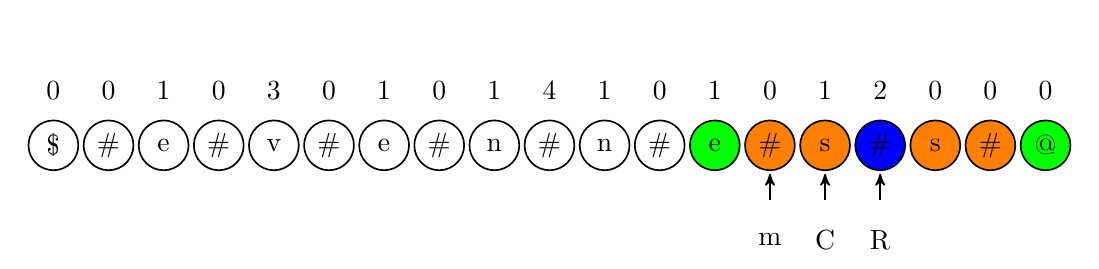
\begin{tikzpicture}[->,>=stealth',shorten >=1pt,auto,node distance=0.7cm,
                    semithick]
\tikzstyle{every state}=[fill=none,draw=black,text=black]
\tikzset{font=\fontsize{10pt}{12}\selectfont}

  
        \node[state,inner sep=2pt,minimum size=18pt]                (0)                           {\$};
        \node[state,inner sep=2pt,minimum size=18pt, draw=none]                (p0) [above of=0] {0};
        
        \node[state,inner sep=2pt,minimum size=18pt]                        (1)   [right of=0]          {\#};
        \node[state,inner sep=2pt,minimum size=18pt, draw=none]                (p1) [above of=1] {0};
        
        \node[state,inner sep=2pt,minimum size=18pt]                        (2)   [right of=1]          {e};
        \node[state,inner sep=2pt,minimum size=18pt, draw=none]                (p2) [above of=2] {1};
        
        \node[state,inner sep=2pt,minimum size=18pt]                        (3)   [right of=2]          {\#};
        \node[state,inner sep=2pt,minimum size=18pt, draw=none]                (p3) [above of=3] {0};
        
        \node[state,inner sep=2pt,minimum size=18pt]              (4)   [right of=3]          {v}; 
        \node[state,inner sep=2pt,minimum size=18pt, draw=none]                (p4) [above of=4] {3};
           
        \node[state,inner sep=2pt,minimum size=18pt]                        (5)   [right of=4]          {\#};
        \node[state,inner sep=2pt,minimum size=18pt, draw=none]                (p5) [above of=5] {0};
        
        \node[state,inner sep=2pt,minimum size=18pt]                        (6)   [right of=5]          {e};
        \node[state,inner sep=2pt,minimum size=18pt, draw=none]                (p6) [above of=6] {1};
        
        \node[state,inner sep=2pt,minimum size=18pt]                        (7)   [right of=6]          {\#};
        \node[state,inner sep=2pt,minimum size=18pt, draw=none]                (p7) [above of=7] {0};
        
        \node[state,inner sep=2pt,minimum size=18pt]              (8)   [right of=7]          {n};
        \node[state,inner sep=2pt,minimum size=18pt, draw=none]                (p8) [above of=8] {1};
            
        \node[state,inner sep=2pt,minimum size=18pt]                        (9)   [right of=8]          {\#};
        \node[state,inner sep=2pt,minimum size=18pt, draw=none]                (p9) [above of=9] {4};
        
        \node[state,inner sep=2pt,minimum size=18pt]                        (10)   [right of=9]          {n};
        \node[state,inner sep=2pt,minimum size=18pt, draw=none]                (p10) [above of=10] {1};
        
        \node[state,inner sep=2pt,minimum size=18pt]                        (11)   [right of=10]          {\#};
        \node[state,inner sep=2pt,minimum size=18pt, draw=none]                (p11) [above of=11] {0};
        
        \node[state,inner sep=2pt,minimum size=18pt, fill=green]                        (12)   [right of=11]          {e};
        \node[state,inner sep=2pt,minimum size=18pt, draw=none]                (p12) [above of=12] {1};
        
        \node[state,inner sep=2pt,minimum size=18pt, fill=orange]                        (13)   [right of=12]          {\#};
        \node[state,inner sep=2pt,minimum size=18pt, draw=none]                (p13) [above of=13] {0};
        
        \node[state,inner sep=2pt,minimum size=18pt, fill=orange]              (14)   [right of=13]          {s};
        \node[state,inner sep=2pt,minimum size=18pt, draw=none]                (p14) [above of=14] {1};
            
        \node[state,inner sep=2pt,minimum size=18pt, fill=blue]                        (15)   [right of=14]          {\#};
        \node[state,inner sep=2pt,minimum size=18pt, draw=none]                (p15) [above of=15] {2};
        
        \node[state,inner sep=2pt,minimum size=18pt, fill=orange]                        (16)   [right of=15]          {s};
        \node[state,inner sep=2pt,minimum size=18pt, draw=none]                (p16) [above of=16] {0};
        
        \node[state,inner sep=2pt,minimum size=18pt, fill=orange]                        (17)   [right of=16]          {\#};
        \node[state,inner sep=2pt,minimum size=18pt, draw=none]                (p17) [above of=17] {0};
        
        \node[state,inner sep=2pt,minimum size=18pt, fill=green]                        (18)   [right of=17]          {@};
        \node[state,inner sep=2pt,minimum size=18pt, draw=none]                (p18) [above of=18] {0};
        
        \node[state,inner sep=2pt,minimum size=28pt,draw=none, node distance = 1.2 cm]	     (C) [below of=14] {C};
        \node[state,inner sep=2pt,minimum size=28pt,draw=none, node distance = 1.2 cm]	     (R) [below of=15] {R};
        \node[state,inner sep=2pt,minimum size=28pt,draw=none, node distance = 1.2 cm]	     (m) [below of=13] {m};        
 
        \path[->]
        (C)   edge node {}            (14)  
        (R)   edge node {}            (15)
        (m)   edge node {}          (13) 
        ; %end path 
        
\end{tikzpicture} 

\\
%---------------------------------------------------------------------------------------------------------------------------------------%
\hline

16 &

~

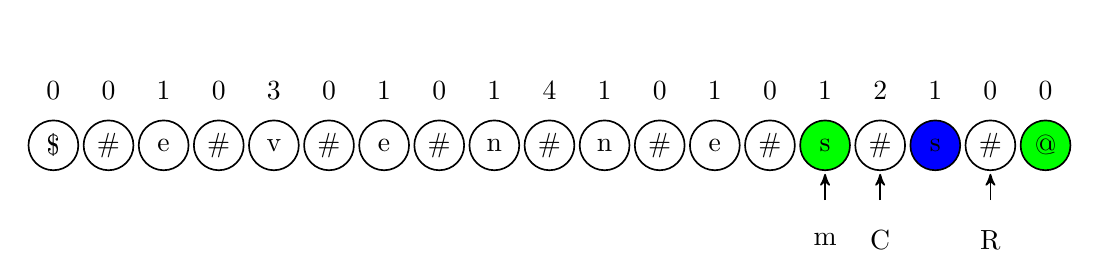
\begin{tikzpicture}[->,>=stealth',shorten >=1pt,auto,node distance=0.7cm,
                    semithick]
\tikzstyle{every state}=[fill=none,draw=black,text=black]
\tikzset{font=\fontsize{10pt}{12}\selectfont}

  
        \node[state,inner sep=2pt,minimum size=18pt]                (0)                           {\$};
        \node[state,inner sep=2pt,minimum size=18pt, draw=none]                (p0) [above of=0] {0};
        
        \node[state,inner sep=2pt,minimum size=18pt]                        (1)   [right of=0]          {\#};
        \node[state,inner sep=2pt,minimum size=18pt, draw=none]                (p1) [above of=1] {0};
        
        \node[state,inner sep=2pt,minimum size=18pt]                        (2)   [right of=1]          {e};
        \node[state,inner sep=2pt,minimum size=18pt, draw=none]                (p2) [above of=2] {1};
        
        \node[state,inner sep=2pt,minimum size=18pt]                        (3)   [right of=2]          {\#};
        \node[state,inner sep=2pt,minimum size=18pt, draw=none]                (p3) [above of=3] {0};
        
        \node[state,inner sep=2pt,minimum size=18pt]              (4)   [right of=3]          {v}; 
        \node[state,inner sep=2pt,minimum size=18pt, draw=none]                (p4) [above of=4] {3};
           
        \node[state,inner sep=2pt,minimum size=18pt]                        (5)   [right of=4]          {\#};
        \node[state,inner sep=2pt,minimum size=18pt, draw=none]                (p5) [above of=5] {0};
        
        \node[state,inner sep=2pt,minimum size=18pt]                        (6)   [right of=5]          {e};
        \node[state,inner sep=2pt,minimum size=18pt, draw=none]                (p6) [above of=6] {1};
        
        \node[state,inner sep=2pt,minimum size=18pt]                        (7)   [right of=6]          {\#};
        \node[state,inner sep=2pt,minimum size=18pt, draw=none]                (p7) [above of=7] {0};
        
        \node[state,inner sep=2pt,minimum size=18pt]              (8)   [right of=7]          {n};
        \node[state,inner sep=2pt,minimum size=18pt, draw=none]                (p8) [above of=8] {1};
            
        \node[state,inner sep=2pt,minimum size=18pt]                        (9)   [right of=8]          {\#};
        \node[state,inner sep=2pt,minimum size=18pt, draw=none]                (p9) [above of=9] {4};
        
        \node[state,inner sep=2pt,minimum size=18pt]                        (10)   [right of=9]          {n};
        \node[state,inner sep=2pt,minimum size=18pt, draw=none]                (p10) [above of=10] {1};
        
        \node[state,inner sep=2pt,minimum size=18pt]                        (11)   [right of=10]          {\#};
        \node[state,inner sep=2pt,minimum size=18pt, draw=none]                (p11) [above of=11] {0};
        
        \node[state,inner sep=2pt,minimum size=18pt]                        (12)   [right of=11]          {e};
        \node[state,inner sep=2pt,minimum size=18pt, draw=none]                (p12) [above of=12] {1};
        
        \node[state,inner sep=2pt,minimum size=18pt]                        (13)   [right of=12]          {\#};
        \node[state,inner sep=2pt,minimum size=18pt, draw=none]                (p13) [above of=13] {0};
        
        \node[state,inner sep=2pt,minimum size=18pt, fill=green]              (14)   [right of=13]          {s};
        \node[state,inner sep=2pt,minimum size=18pt, draw=none]                (p14) [above of=14] {1};
            
        \node[state,inner sep=2pt,minimum size=18pt]                        (15)   [right of=14]          {\#};
        \node[state,inner sep=2pt,minimum size=18pt, draw=none]                (p15) [above of=15] {2};
        
        \node[state,inner sep=2pt,minimum size=18pt, fill=blue]                        (16)   [right of=15]          {s};
        \node[state,inner sep=2pt,minimum size=18pt, draw=none]                (p16) [above of=16] {1};
        
        \node[state,inner sep=2pt,minimum size=18pt]                        (17)   [right of=16]          {\#};
        \node[state,inner sep=2pt,minimum size=18pt, draw=none]                (p17) [above of=17] {0};
        
        \node[state,inner sep=2pt,minimum size=18pt, fill=green]                        (18)   [right of=17]          {@};
        \node[state,inner sep=2pt,minimum size=18pt, draw=none]                (p18) [above of=18] {0};
        
        \node[state,inner sep=2pt,minimum size=28pt,draw=none, node distance = 1.2 cm]	     (C) [below of=15] {C};
        \node[state,inner sep=2pt,minimum size=28pt,draw=none, node distance = 1.2 cm]	     (R) [below of=17] {R};
        \node[state,inner sep=2pt,minimum size=28pt,draw=none, node distance = 1.2 cm]	     (m) [below of=14] {m};        
 
        \path[->]
        (C)   edge node {}            (15)  
        (R)   edge node {}            (17)
        (m)   edge node {}          (14) 
        ; %end path 
        
\end{tikzpicture} 

\\
%---------------------------------------------------------------------------------------------------------------------------------------%
\hline

17 &

~

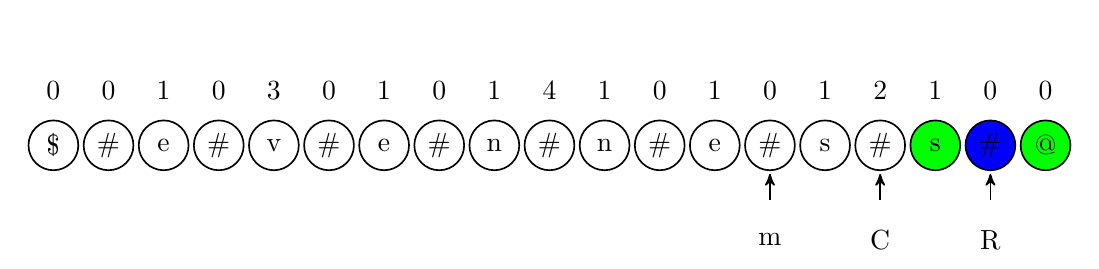
\begin{tikzpicture}[->,>=stealth',shorten >=1pt,auto,node distance=0.7cm,
                    semithick]
\tikzstyle{every state}=[fill=none,draw=black,text=black]
\tikzset{font=\fontsize{10pt}{12}\selectfont}

  
        \node[state,inner sep=2pt,minimum size=18pt]                (0)                           {\$};
        \node[state,inner sep=2pt,minimum size=18pt, draw=none]                (p0) [above of=0] {0};
        
        \node[state,inner sep=2pt,minimum size=18pt]                        (1)   [right of=0]          {\#};
        \node[state,inner sep=2pt,minimum size=18pt, draw=none]                (p1) [above of=1] {0};
        
        \node[state,inner sep=2pt,minimum size=18pt]                        (2)   [right of=1]          {e};
        \node[state,inner sep=2pt,minimum size=18pt, draw=none]                (p2) [above of=2] {1};
        
        \node[state,inner sep=2pt,minimum size=18pt]                        (3)   [right of=2]          {\#};
        \node[state,inner sep=2pt,minimum size=18pt, draw=none]                (p3) [above of=3] {0};
        
        \node[state,inner sep=2pt,minimum size=18pt]              (4)   [right of=3]          {v}; 
        \node[state,inner sep=2pt,minimum size=18pt, draw=none]                (p4) [above of=4] {3};
           
        \node[state,inner sep=2pt,minimum size=18pt]                        (5)   [right of=4]          {\#};
        \node[state,inner sep=2pt,minimum size=18pt, draw=none]                (p5) [above of=5] {0};
        
        \node[state,inner sep=2pt,minimum size=18pt]                        (6)   [right of=5]          {e};
        \node[state,inner sep=2pt,minimum size=18pt, draw=none]                (p6) [above of=6] {1};
        
        \node[state,inner sep=2pt,minimum size=18pt]                        (7)   [right of=6]          {\#};
        \node[state,inner sep=2pt,minimum size=18pt, draw=none]                (p7) [above of=7] {0};
        
        \node[state,inner sep=2pt,minimum size=18pt]              (8)   [right of=7]          {n};
        \node[state,inner sep=2pt,minimum size=18pt, draw=none]                (p8) [above of=8] {1};
            
        \node[state,inner sep=2pt,minimum size=18pt]                        (9)   [right of=8]          {\#};
        \node[state,inner sep=2pt,minimum size=18pt, draw=none]                (p9) [above of=9] {4};
        
        \node[state,inner sep=2pt,minimum size=18pt]                        (10)   [right of=9]          {n};
        \node[state,inner sep=2pt,minimum size=18pt, draw=none]                (p10) [above of=10] {1};
        
        \node[state,inner sep=2pt,minimum size=18pt]                        (11)   [right of=10]          {\#};
        \node[state,inner sep=2pt,minimum size=18pt, draw=none]                (p11) [above of=11] {0};
        
        \node[state,inner sep=2pt,minimum size=18pt]                        (12)   [right of=11]          {e};
        \node[state,inner sep=2pt,minimum size=18pt, draw=none]                (p12) [above of=12] {1};
        
        \node[state,inner sep=2pt,minimum size=18pt]                        (13)   [right of=12]          {\#};
        \node[state,inner sep=2pt,minimum size=18pt, draw=none]                (p13) [above of=13] {0};
        
        \node[state,inner sep=2pt,minimum size=18pt]              (14)   [right of=13]          {s};
        \node[state,inner sep=2pt,minimum size=18pt, draw=none]                (p14) [above of=14] {1};
            
        \node[state,inner sep=2pt,minimum size=18pt]                        (15)   [right of=14]          {\#};
        \node[state,inner sep=2pt,minimum size=18pt, draw=none]                (p15) [above of=15] {2};
        
        \node[state,inner sep=2pt,minimum size=18pt, fill=green]                        (16)   [right of=15]          {s};
        \node[state,inner sep=2pt,minimum size=18pt, draw=none]                (p16) [above of=16] {1};
        
        \node[state,inner sep=2pt,minimum size=18pt, fill=blue]                        (17)   [right of=16]          {\#};
        \node[state,inner sep=2pt,minimum size=18pt, draw=none]                (p17) [above of=17] {0};
        
        \node[state,inner sep=2pt,minimum size=18pt, fill=green]                        (18)   [right of=17]          {@};
        \node[state,inner sep=2pt,minimum size=18pt, draw=none]                (p18) [above of=18] {0};
        
        \node[state,inner sep=2pt,minimum size=28pt,draw=none, node distance = 1.2 cm]	     (C) [below of=15] {C};
        \node[state,inner sep=2pt,minimum size=28pt,draw=none, node distance = 1.2 cm]	     (R) [below of=17] {R};
        \node[state,inner sep=2pt,minimum size=28pt,draw=none, node distance = 1.2 cm]	     (m) [below of=13] {m};        
 
        \path[->]
        (C)   edge node {}            (15)  
        (R)   edge node {}            (17)
        (m)   edge node {}          (13) 
        ; %end path 
        
\end{tikzpicture} 

\\

\hline
\end{tabular}
\end{center}

%----------------------------------------------------------------------------------------
\end{document}